\documentclass{article}

\usepackage{graphicx}
\usepackage[utf8]{inputenc}
\usepackage[hmargin=2.5cm,vmargin=2.5cm]{geometry}
\usepackage[section]{placeins}
\usepackage[french]{babel} 
\usepackage{subcaption}
\usepackage{titlesec}
\setcounter{secnumdepth}{4}
\setcounter{tocdepth}{4}

\titleformat{\paragraph}
{\normalfont\normalsize\bfseries}{\theparagraph}{1em}{}
\titlespacing*{\paragraph}
{0pt}{3.25ex plus 1ex minus .2ex}{1.5ex plus .2ex}

\newcommand{\rapportFigure}{0.075}
\newcommand{\rapportSubFigure}{0.069}

\title{Stage Ouvrier}
\author{Gustavo Ciotto Pinton}
\date{September 2014}

\begin{document}

\begin{titlepage}
\vspace*{.18\textheight}
\begin{center}
%
\begin{figure}[h]
    \centering
    
\includegraphics[scale=0.12]{images/LogoSupelec}\\
    
\includegraphics[scale=0.5]{images/LogoElis}
\end{figure}
%
\vspace*{10pt}
%\text{ }\\[7 cm]
\textbf{\LARGE 1re ANNEE D'ECOLE D'INGENIEUR} \\[0.5 cm]
\textbf{\LARGE STAGE D'EXECUTION}\\[1 cm]

Gustavo \textbf{CIOTTO PINTON}\\
Promotion 2013-2015\\[1 cm]

M. Guillaume \textbf{BRAURE}\\
Chef de Production - Elis Brétigny\\[1 cm]

Du 11 Juillet 2014 au 14 Septembre 2014

\end{center}
\end{titlepage}

\newpage
\tableofcontents

\newpage
\section*{Remerciements}
\addcontentsline{toc}{section}{Remerciements}

Cette section du rapport est specialement dédiée à toutes les personnes qui
m'ont aidé à bien réussir ma première expérience professionelle et
internationalle, et envers qui je suis vraiment reconnaissant.

\vspace{12pt}

Tout d'abord, je remercie toute la diréction de l'Ecole, specialement
Madame Guessab qui a été toujours là pour répondre mes questions et à
m'orienter, et surtout tous les professeurs qui composent le corps enseignant,
en particulier Monsieur Benadon et Madame Cherbal qui m'ont aidé à construire
et traduire mon CV et ma lettre de motivation.

\vspace{12pt}

Et enfin, je remercie tous mes collègues de travail, sans lesquels je
n'aurais pas eu réussit à surmonter les défis presentés tous les jours
durant les derniers deux mois. Particulièrement, je remercie tous les chefs
d'équipe, specialement Monsieur Braure et Monsieur Hebting, qui ont toujours su 
être patients et gentils face aux bêtises parfois réalisées.


\newpage
\section{Introduction}

Les éléves d'une grande école, telle comme Supélec, sont constamment amenés à
prendre des décisions et à penser comme de vrais chefs ou des directeurs
d'entreprises. Par conséquent, nous sommes invités à penser à notre avenir
professionnel dès nos premiers jours au sein de cette Ecole. Compte tenu de ces
caractéristiques, une expérience concrète après la première année se présente
comme une opportunité très particulière pour renforcer ou changer des concepts
et projets,  acquies et élaborés pendant les cours à Supélec. Le stage
d'éxécution, realisé en milieu industriel, est ainsi une opportunité qui leur
offre des enseignements fondamentaux à la construction d'une carrière solide.

\vspace{12pt}

Personnellement, je me suis interessé principalement à ce type de stage parce
que, comme un éleve étranger, j'avais envie - et un peu de curiosité aussi - de
travailler dans une entreprise internationale. Je voulais savoir comment je
serais perçu par les autres, comment serait la communication voire si elle
serait possible. En outre, l'un des facteurs qui m'a fait choisir la France
pour continuer mes études a été précisément la possibilité de bien y construire
une carrière professionelle.

\vspace{12pt}

En ce qui concerne l'entreprise, Elis a comme métier surtout la
location-entretien de vêtements professionnels et de linge, mais offre aussi
des services complémentaires tels que les fontaines à eau, les tapis et les
équipements sanitaires. Le groupe opère en Europe et a acheté récemment une
filiale au Brésil, ce qui peut répresenter une possible opportunité dans
l'avenir.

\vspace{12pt}

Mon stage comme opérateur de production a eu lieu au centre de
Brétigny-sur-Orge, du 11 Juillet au 14 Septembre, sous la responsabilité de M.
Braure et M. Hebting. J'ai été responsable sur plusieurs missions pendant ces
deux mois, ce qui m'a apporté des connaissances par rapport au fonctionnement
de toute l'usine. Les termes et conditions de travail ont été accordés après la
convention de stage et l'entretien, comme par exemple les horaires d'entrée et
de sortie, étant respectivement 12h30 et 20h05. En outre, j'ai eu à travailler
tous les samedis et jours feriés.

\vspace{12pt}

Quant aux tâches effectuées seront mieux detaillés dans la suite du
document, ainsi comme mes réflexions vis-à-vis mon séjour chez Elis.

\newpage
\section{L'entreprise}

Cette section porte sur l'entreprise dans laquelle le stage a été éffectué. Tout
d'abord, je vous présente la structure générale du groupe Elis - son identité,
historique - et après l'organisation spécifique de l'usine de Brétigny -
secteurs, hiérarchie etc. A la fin, je vous presente le processus d'embauche,
ainsi qu'un descriptif de journée durant ces deux derniers mois.

\subsection{Présentation générale du groupe Elis}

Le groupe Elis s'engage à offrir une grande gamme de services à des entreprises
dans plusieurs secteurs d'économie. Son objectif principal est de \og
simplifier la vie entreprises quels que soient leur taille ou domaine
d'activité afin qu'elles puissent se recentrer sur leur métier \fg~. C'est
grâce à cette détermination que le groupe présente l'évolution et la croissance
qui peuvent être traduits par certains chiffres: aujourd'hui il possède 18.500
collaborateurs dans toute l'Europe - dont 11.500 en France - et au Brésil, 256
centres de service et production, plus de 240.00 clients de toutes tailles et
secteurs et un chiffre d'affaires toujours en  progression depuis 40 ans.

\vspace{12pt}

Creé en 1968, le groupe est responsable de nombreux services, parmi
lesquels on cite principalement l'habillement professionnel, le linge de
restauration et d'hébergement, le linge de santé, l'hygiène des sanitaires, la
protection des sois et service boisson, y compris les fontaines à bonbonne, les
fontaines réseaux et machines à café.

\subsection{Présentation du centre de Brétigny}

Le centre de Brétigny est spécialisé dans le linge de restauration et le linge
d'hébergement utilisés dans plusieurs établissements en Ile-de-France. Par
con\-séquent, en raison de la grande quantité qui doit être traité afin
de respecter les délais et qualité éxigés, l'usine compte
sur des équipements et outils d'haute précision et performance. Quant à
l'organisation, elle est divisée en 5 secteurs, y compris l'hébergement, la
restauration, le contrôle entrée, les bobines et la rénovation.

\vspace{12pt}

Son fonctionnement suit notamment un cycle composé de 6 étapes principales.
Tout d'abord, l'entreprise s'engage à ramasser le linge sale chez nos clients.
Les produits passent pour un premier contrôle lors de leur arrivée, qui
consiste essentiellement à trier les différentes catégories des draps, housses,
draps de bains, éponges etc, exigeant ainsi des opérateurs une connaissance
solide des pièces. Le linge trié est alors lavé (troisième étape), séché,
repassé et plié (quatrième) et finalement mis au contrôle de qualité et à
l'expédition (cinquième). Les derniers sont responsables pour préparer les
commandes spécifiques de chaque client, à l'aide des fiches contenant les
quantités des produits respectifs. Enfin, le linge est livré et le cycle peut
recommencer à nouveau.

\vspace{12pt}

A propos de l'organisation hiérarchique, le centre de Brétigny compte sur son
directeur, le poste le plus haut , pour bien l'administrer. Ensuite, chacun
des secteurs de l'usine possède un chef de ligne, dont la principale fonction
est de construire des plannings et assurer qu'ils soient bien suivis par les
opérateurs. Ils sont responsables aussi du bon fonctionnement des machines
et l'avancement général de l'usine. Après, les chefs d'équipe aident le chef de
ligne à atteindre ses objectifs, en gérant des groupes plus petits et en
s'assurant de la qualité et la performance du service. Et enfin, chaque poste a
un chef - généralement un opérateur plus expérimenté - qui veille à son bon
déroulement.

\vspace{12pt}

Quant aux autres aspects, il existe des équipements de protection individuelle,
comme des gants, blouses et chaussures de sécurité, sont obligatoires puisqu'il
s'agit d'un milieu industriel.

\vspace{12pt}

En ce qui concerne les horaires et jours de travail, le service de production
reste ouvert du lundi au samedi, ainsi que les jours fériés. Il est composé de
deux équipes: une le matin, de 5h55 à 13h30, et une l'après midi, de 13h30 à
21h05. Les équipes disposent d'une pause de 20 minutes.

\subsection{La recherche et le processus d'embauche}

Dans un premier temps, j'ai basé mes recherches de stage sur les contacts des
entreprises présentées dans le livre du Forum. Le seul résultat concret que
j'ai obtenu a été un entretien téléphonique avec Valeo. Par la suite, j'ai
essayé d'élargir mes recherches en postulant ma candidature sur des sites
spécialisés, comme, par exemple, l'Etudiant.fr et indeed.fr.

\vspace{12pt}

Une des entreprises, appelée Littlebig Road, m'a contacté et m'a proposé un
stage du 1er août au 15 septembre.
Malheureusement, je n'ai pas pu accepter cette offre, car les cours
recommenceraient précisément à la fin du stage. Afin de changer de période et
faire possible que cela soit possible, je leur ai envoyé un email proposant
une modification, mais je n'ai aucune résponse.

\vspace{12pt}

Mes espoirs étaient presque épuisées lorsque j'ai finalement reçu une offre
concrète venue de mon futur maître de stage, M. Braure. Il s'agissait d'une des
offres à laquelle j'avais postulées sur ligne. Ensuite, après avoir été
contacté par téléphone, j'ai passé par une entretien d'embauche, qui
dans un premier temps m'a fait un peu peur, alors qu'habituellement je ne parle
pas français couramment. Cependant, j'ai reússi a remplacer mon handicap par une
bonne et solide préparation, basée sur des recherches realisées sur le site de
l'entreprise, et en conséquence j'ai été embauché.

\vspace{12pt}

Par rapport à l'entretien, les principales questions posées concernaient les
raisons de mon choix de continuer mes études en France et principalement ce
que j'attendais de mon stage chez Elis. Malheuseument, il ne m'a jamais été
mentionné lors de l'entretien que j'aurais à travailler les samedis et  les
jours feriés, ce qui m'a rendu un peu déçu car je n'en avais pas été informé
préalablement par la RH. Sincèrement, j'aurais de grosses doutes à accepter de 
telles conditions si je n'avais pas être obligé de faire un stage ouvrier.
Cependant, j'étais très motivé et cela m'a encouragé à continuer le stage
même avec ces défis.

\vspace{12pt}

Le processus s'est finalement terminé après que toutes les parties - moi, la
diréction de l'école et l'entreprise - avion  signé la convention de stage. Je
faisais partie donc de l'équipe de l'après midi du secteur d'hébergement du 11
juillet au 14 septembre. En fait, compte tenu du dernier bus avec pour 
\og Moulon\fg~ à 21h45, j'ai proposé que mes horaires d'entrée et sortie soient
avancés d'une heure, devenant ainsi respectivement 12h30 et 20h05.  J'étais
alors prêt à commencer cette nouvelle expérience!

\subsection{Mon quotidien}

Ma journée commençait à 10h avec la prise du premier bus à l'arrêt \og
Moulon \fg~ jusqu'à la gare de Massy Palaiseau, où je prennais le premier
train à 10h38, le RER C vers \og Versailles Chatêau Rive Gauche \fg. Après cinq
arrêts - Longjumeau, Chilly Mazarin, Gravigny Mazarin et Petit Vaux - j'arrive à
la gare de Savigny-sur-Orge, où je dois prendre mon deuxième train avec
direction à \og Dourdan la Forêt \fg~ à 11h08 jusqu'à Brétigny-sur-Orge,
passant par les arrêts d'Épinay-sur-Orge, Ste-Généviève-des-Bois et
St-Michel-sur-Orge. Le dernier bus me conduit à l'entreprise et part à 11h25, y
arrivant à 11h35.

\vspace{12pt}

Je prends mon déjeuner et commence à travailler à 12h30 jusqu'à 18h, l'horaire
de début de la pause de 20 minutes. Enfin, je continue jusqu'à 20h05. Les
résultats\footnote{Regardez la section \ref{sec:resultat} pour plus de
informations} du jour précédent sont préséntés et analysés par le chef à
l'équipe tout d'abord.

\vspace{12pt}

Le voyage de retour commence à partir de l'entreprise à 20h14. J'arrive à la
gare de Brétigny à 20h30 et, par train, à Savigny-sur-Orge à 20h43. Finalement,
je prends le dernier train vers Massy Palaiseau à 21h03 et le bus vers Supélec
à 21h45, pour enfin arriver à 22h05 chez moi.

\vspace{12pt}

A mon avis, l'aspect le plus difficile a été précisément les transports. Outre
le temps perdu tous les jours - environ 3 heures et demi chaque jour -, la
dépendance aux transports publics, soit le bus, soit le réseau ferroviaire, a
rendu mes journées plus fatigantes et stressantes en raison des nombreuses \oe
uvres sur l'infrastructure deployées par SNCF et RATP. C'est possible citer par
exemple les récentes modifications de la ligne 91.10, qui m'oblige à marcher à
pied le chemin entre l'arrêt provisoire Corbeville et Supélec tous les soirs,
et l'incendie du poste de Vitry-sur-Seine qui, à son tour, a causé de
suppressions et changements sur les lignes SCNF. En bref, les occasions au cours
desquelles j'ai eu à marcher de la gare \og le Guichet\fg~ jusqu'à
l'école se sont répétés certaines fois pendant cette période.

\vspace{12pt}

Il faut dire aussi que j'avais un \og jour de repos\fg~, choisi
en fonction des demandes hebdomadaires, durant toutes les semaines, où je ne
travaillais pas. Cela me permettait de remplacer les samedis.


\section{Activités effectuées pendant le stage}

Ensuite dans les prochaines sections, les activités qui ont été proposées
pendant le stage sont expliquées et mieux detaillées.

\subsection{Contrôle Entrée}


Le linge sale vient des clients et nécessite d'être préparé avant qu'il ne suive
d'autres secteurs. Le \og contrôle entrée \fg~est alors responsable pour tâches
comme le tri et la récéption du linge qui sont miex décrites dans les sections
suivantes. La figure \ref{fig:entree} montre un des postes de travail du secteur
en question dont l'usage est de trier le linge. Les opérateurs restent sur la
plate-forme et les pièces arrivent à travers un tapis, situé tout au fond de
l'image. Le principle est alors de mettre chaque type de linge dans un chariot
distinct, selon les étiquettes.
%
\begin{figure}[h]
    \centering
    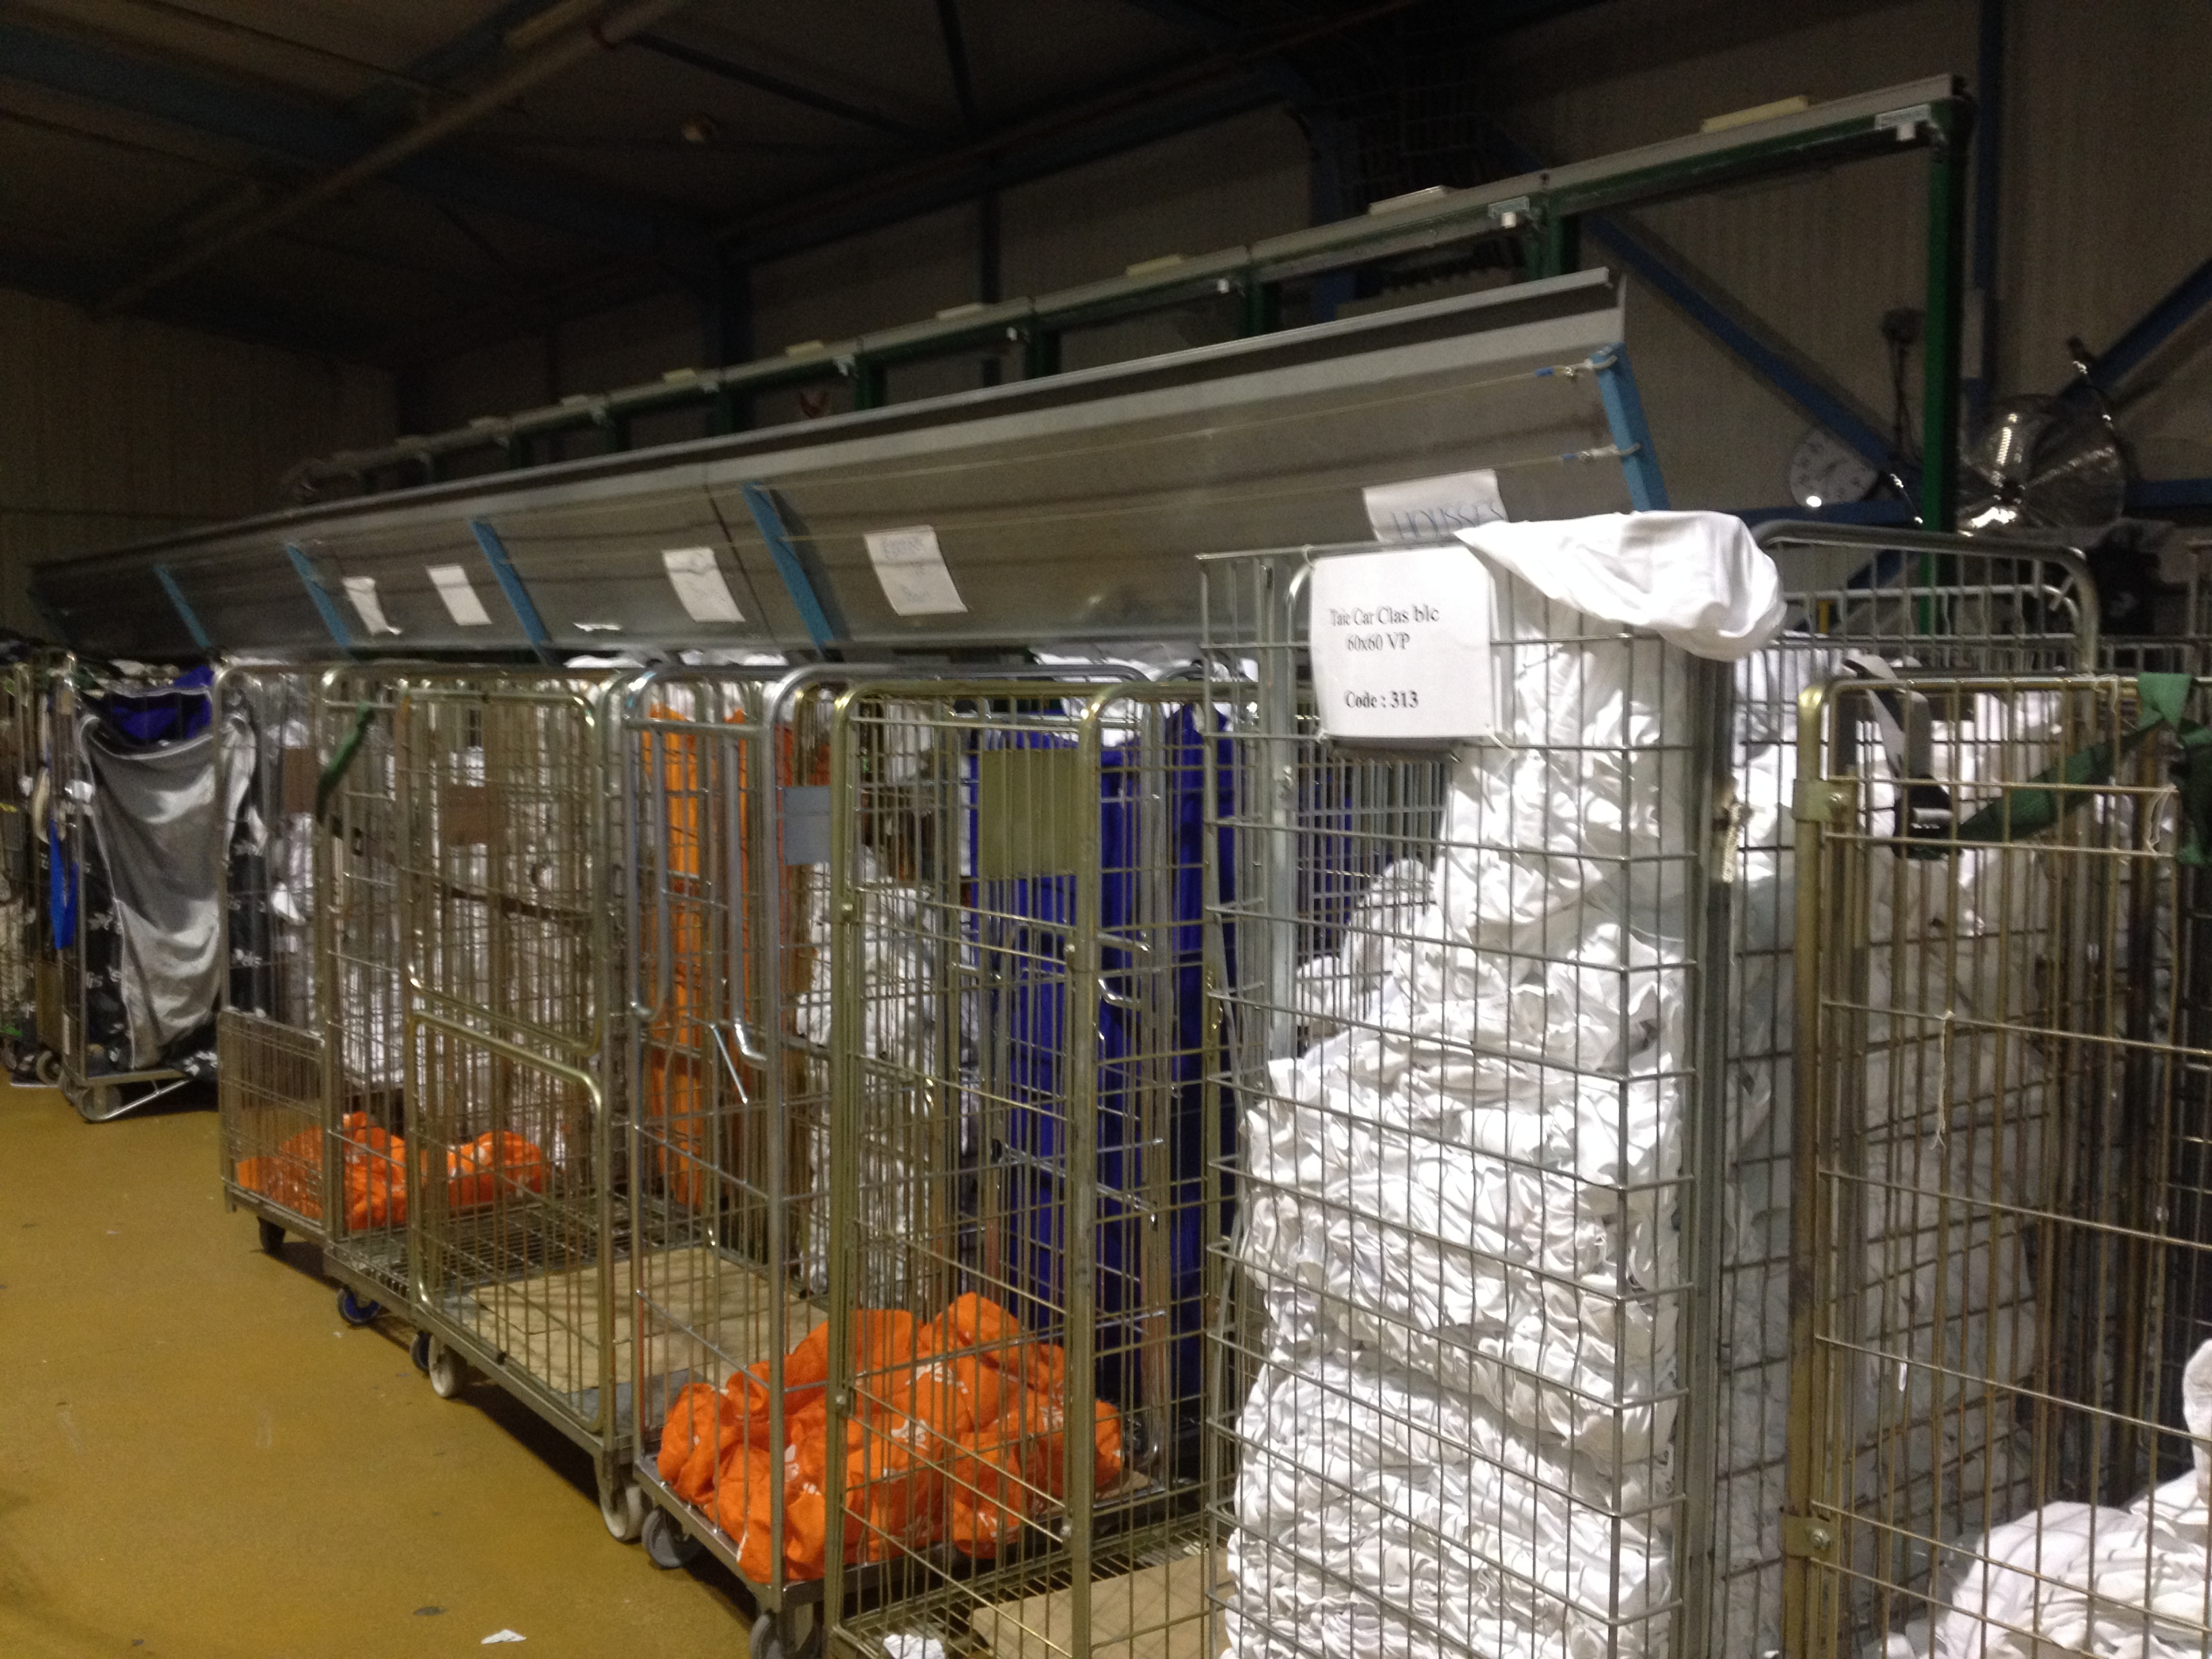
\includegraphics[scale= \rapportFigure]{images/entree}
    \caption{Contrôle entrée.}
    \label{fig:entree}
\end{figure}
%


\subsubsection{Engagement du linge}

Cette première étape consiste à un opérateur engager le linge qui arrive des
clients sur le tapis, afin que ses collègues de travail puissent mieux
identifier les différentes pièces et ainsi les trier plus efficacement.

\subsubsection{Tri du linge}

Les opérateurs qui travaillent sur la plate-forme sont responsables pour
récuperer le linge du tapis et les mettre dans le chariot, selon la
figure \ref{fig:entree_tri}. On remarque aussi les étiquettes - tapis, éponges
par exemple - sur les chariots.

\FloatBarrier

%
\begin{figure}[h]
    \centering
    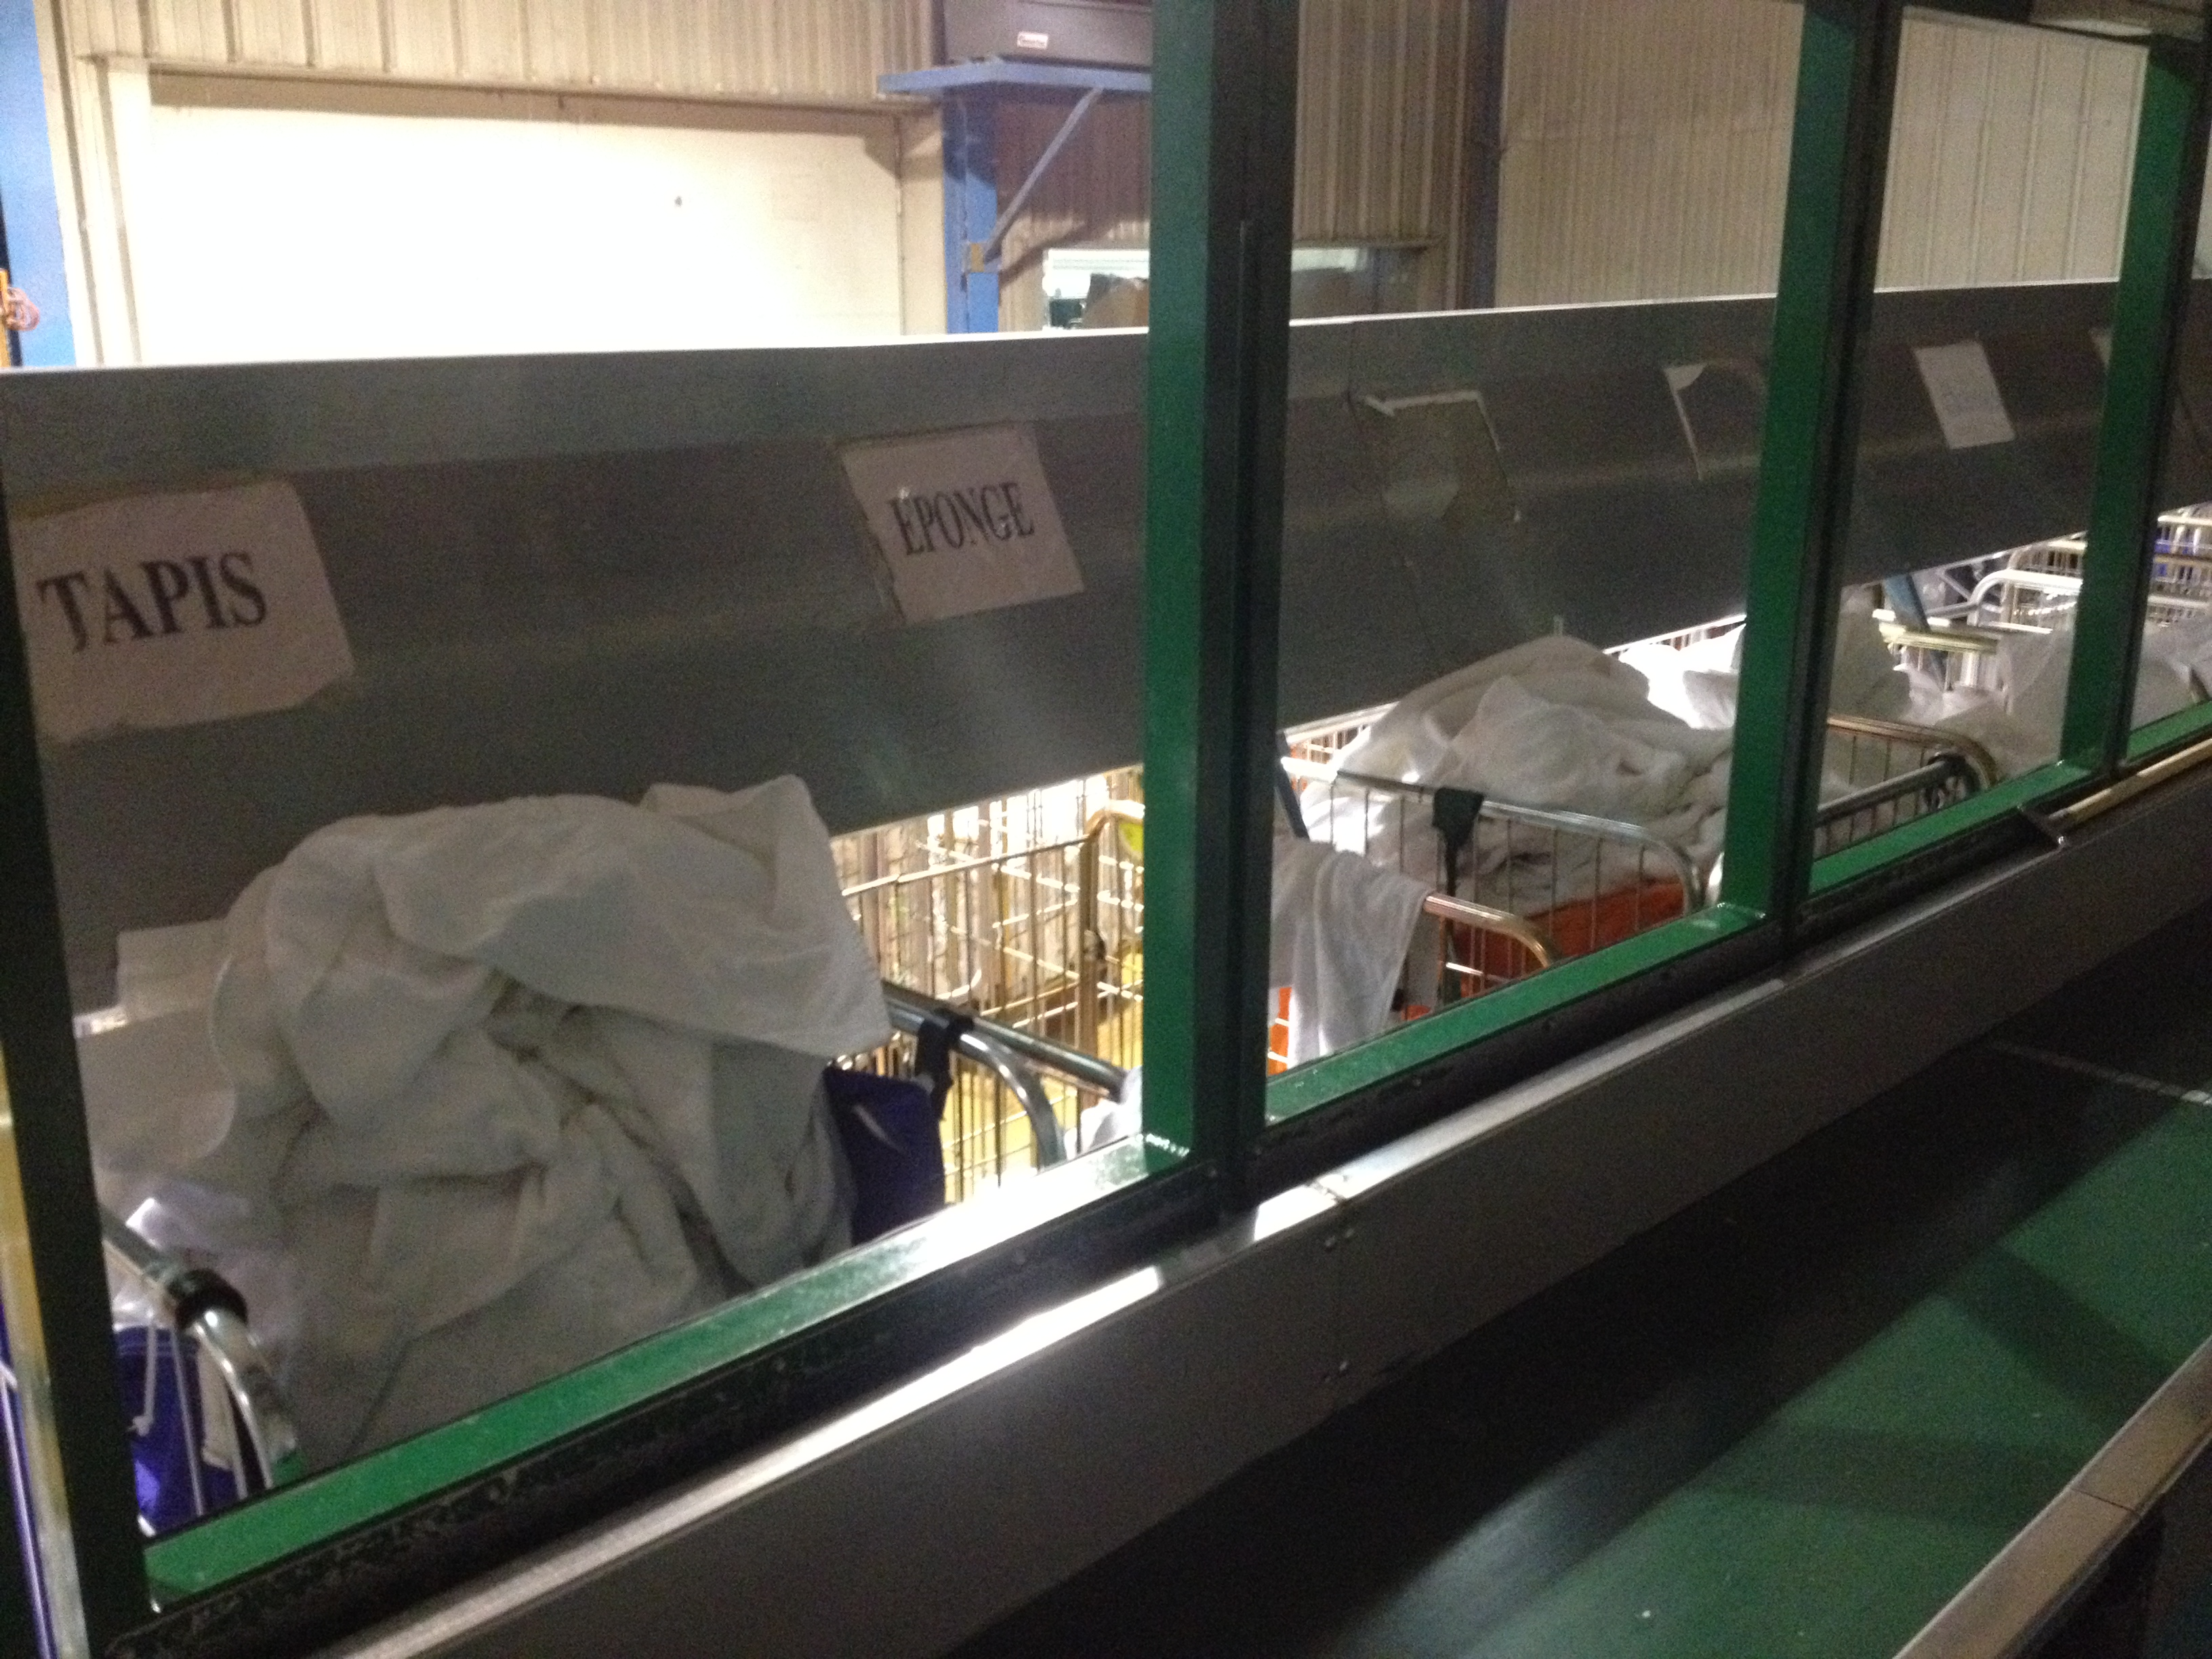
\includegraphics[scale= \rapportFigure]{images/entree_tri}
    \caption{Tri du linge au contrôle entrée.}
    \label{fig:entree_tri}
\end{figure}
%
\FloatBarrier

\subsection{Hébergement}

Cette section est dédiée au secteur d'hébergement responsable de toutes les
commandes des draps, housses, éponges etc. C'est aussi le secteur où je suis
resté la plupart du temps et, par conséquent, développé plus d'activités.

\subsubsection{Résultats du jour}
\label{sec:resultat}

Avant le début des opérations de chaque équipe, le chef présente et commente
les résultats du jour précédent à l'aide d'un tableau, vu en figure
\ref{fig:tableau}. Les lignes répresent les machines et les colonnes, chacun
des aspects analysés. La première moitié des colonnes concernent l'équipe du
matin et la deuxième à cette de l'après-midi. La première colonne, écrite en
noir, est utilisée pour montrer l'efficacité de référence attendue par les chefs
pour chaque machine. Cette efficacité, apellée aussi \textit{TRG}, ne compte que les
périodes où la machine opére. Ainsi, des pannes ou ârrets ne sont pas
considérés dans ce calcul. La colonne suivante, \textit{TRG J}, montre ce qui a
été atteint par l'équipe et est marquée d'une couleur: les résultats négatifs
sont écrits en rouge et les positifs en vert . Enfin, la dernière colonne prend en
compte tous les aléas et ârrets des machines.

\FloatBarrier

%
\begin{figure}[h]
    \centering
    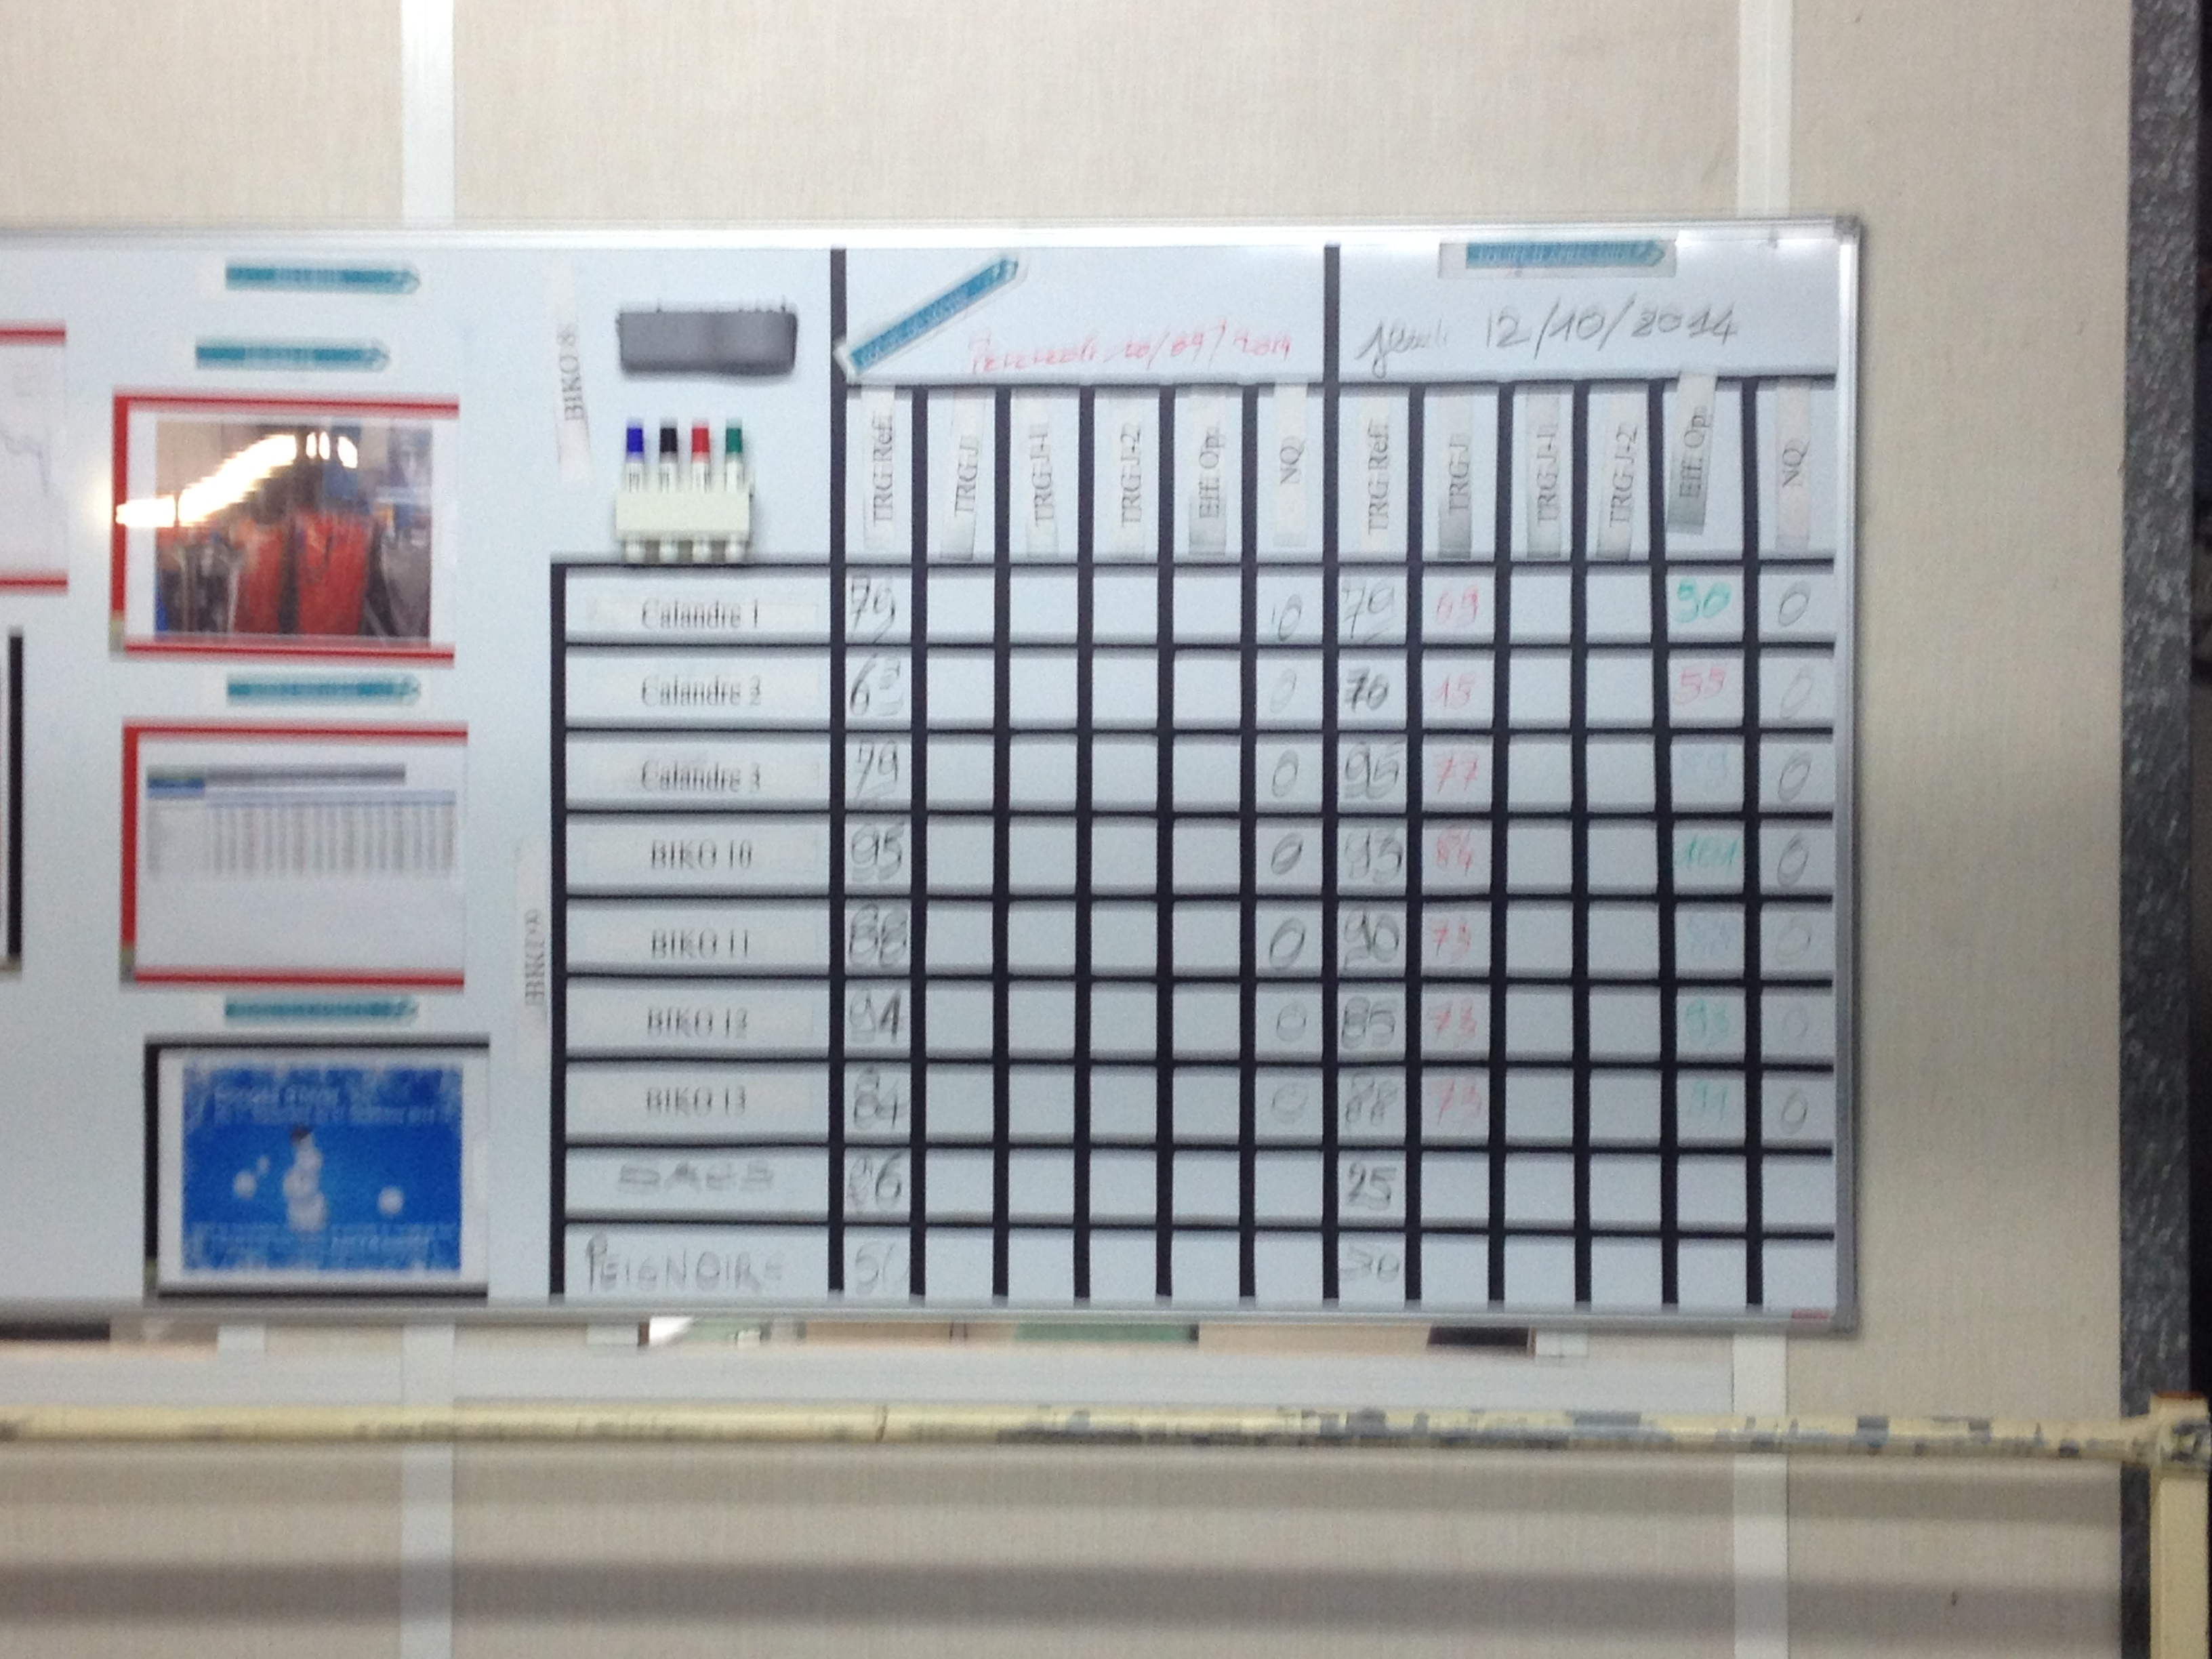
\includegraphics[scale= \rapportFigure]{images/quadre_jour}
    \caption{Résultats du jour précédent affichés sur le tableau.}
    \label{fig:tableau}
\end{figure}
%
\FloatBarrier

\subsubsection{Engagement du linge - les calandres}

La figure \ref{fig:calandre} montre une des calandres. On remarque la présence
d'un écran, figure \ref{fig:ecran} au poste plus à droite, dont finalité
consiste à afficher les résultats - voir section \ref{sec:resultat} - et
permettre l'opérateur responsable de qualifier une possible interruption que la
machine puisse avoir, par exemple, un éventuel probleme mécanique. On note
encore la présence d'un graphique de la quantité des pièces engagées en
fonction du temps avec trois lignes: celle la plus supérieure, en bleue,
répresente l'objectif. La deuxième, en verte, l'objectif hors aléas et
finalement, en rose, l'efficience réelle.

\FloatBarrier
%
\begin{figure}[ht]
    \centering
    \begin{subfigure}{0.49\textwidth}
        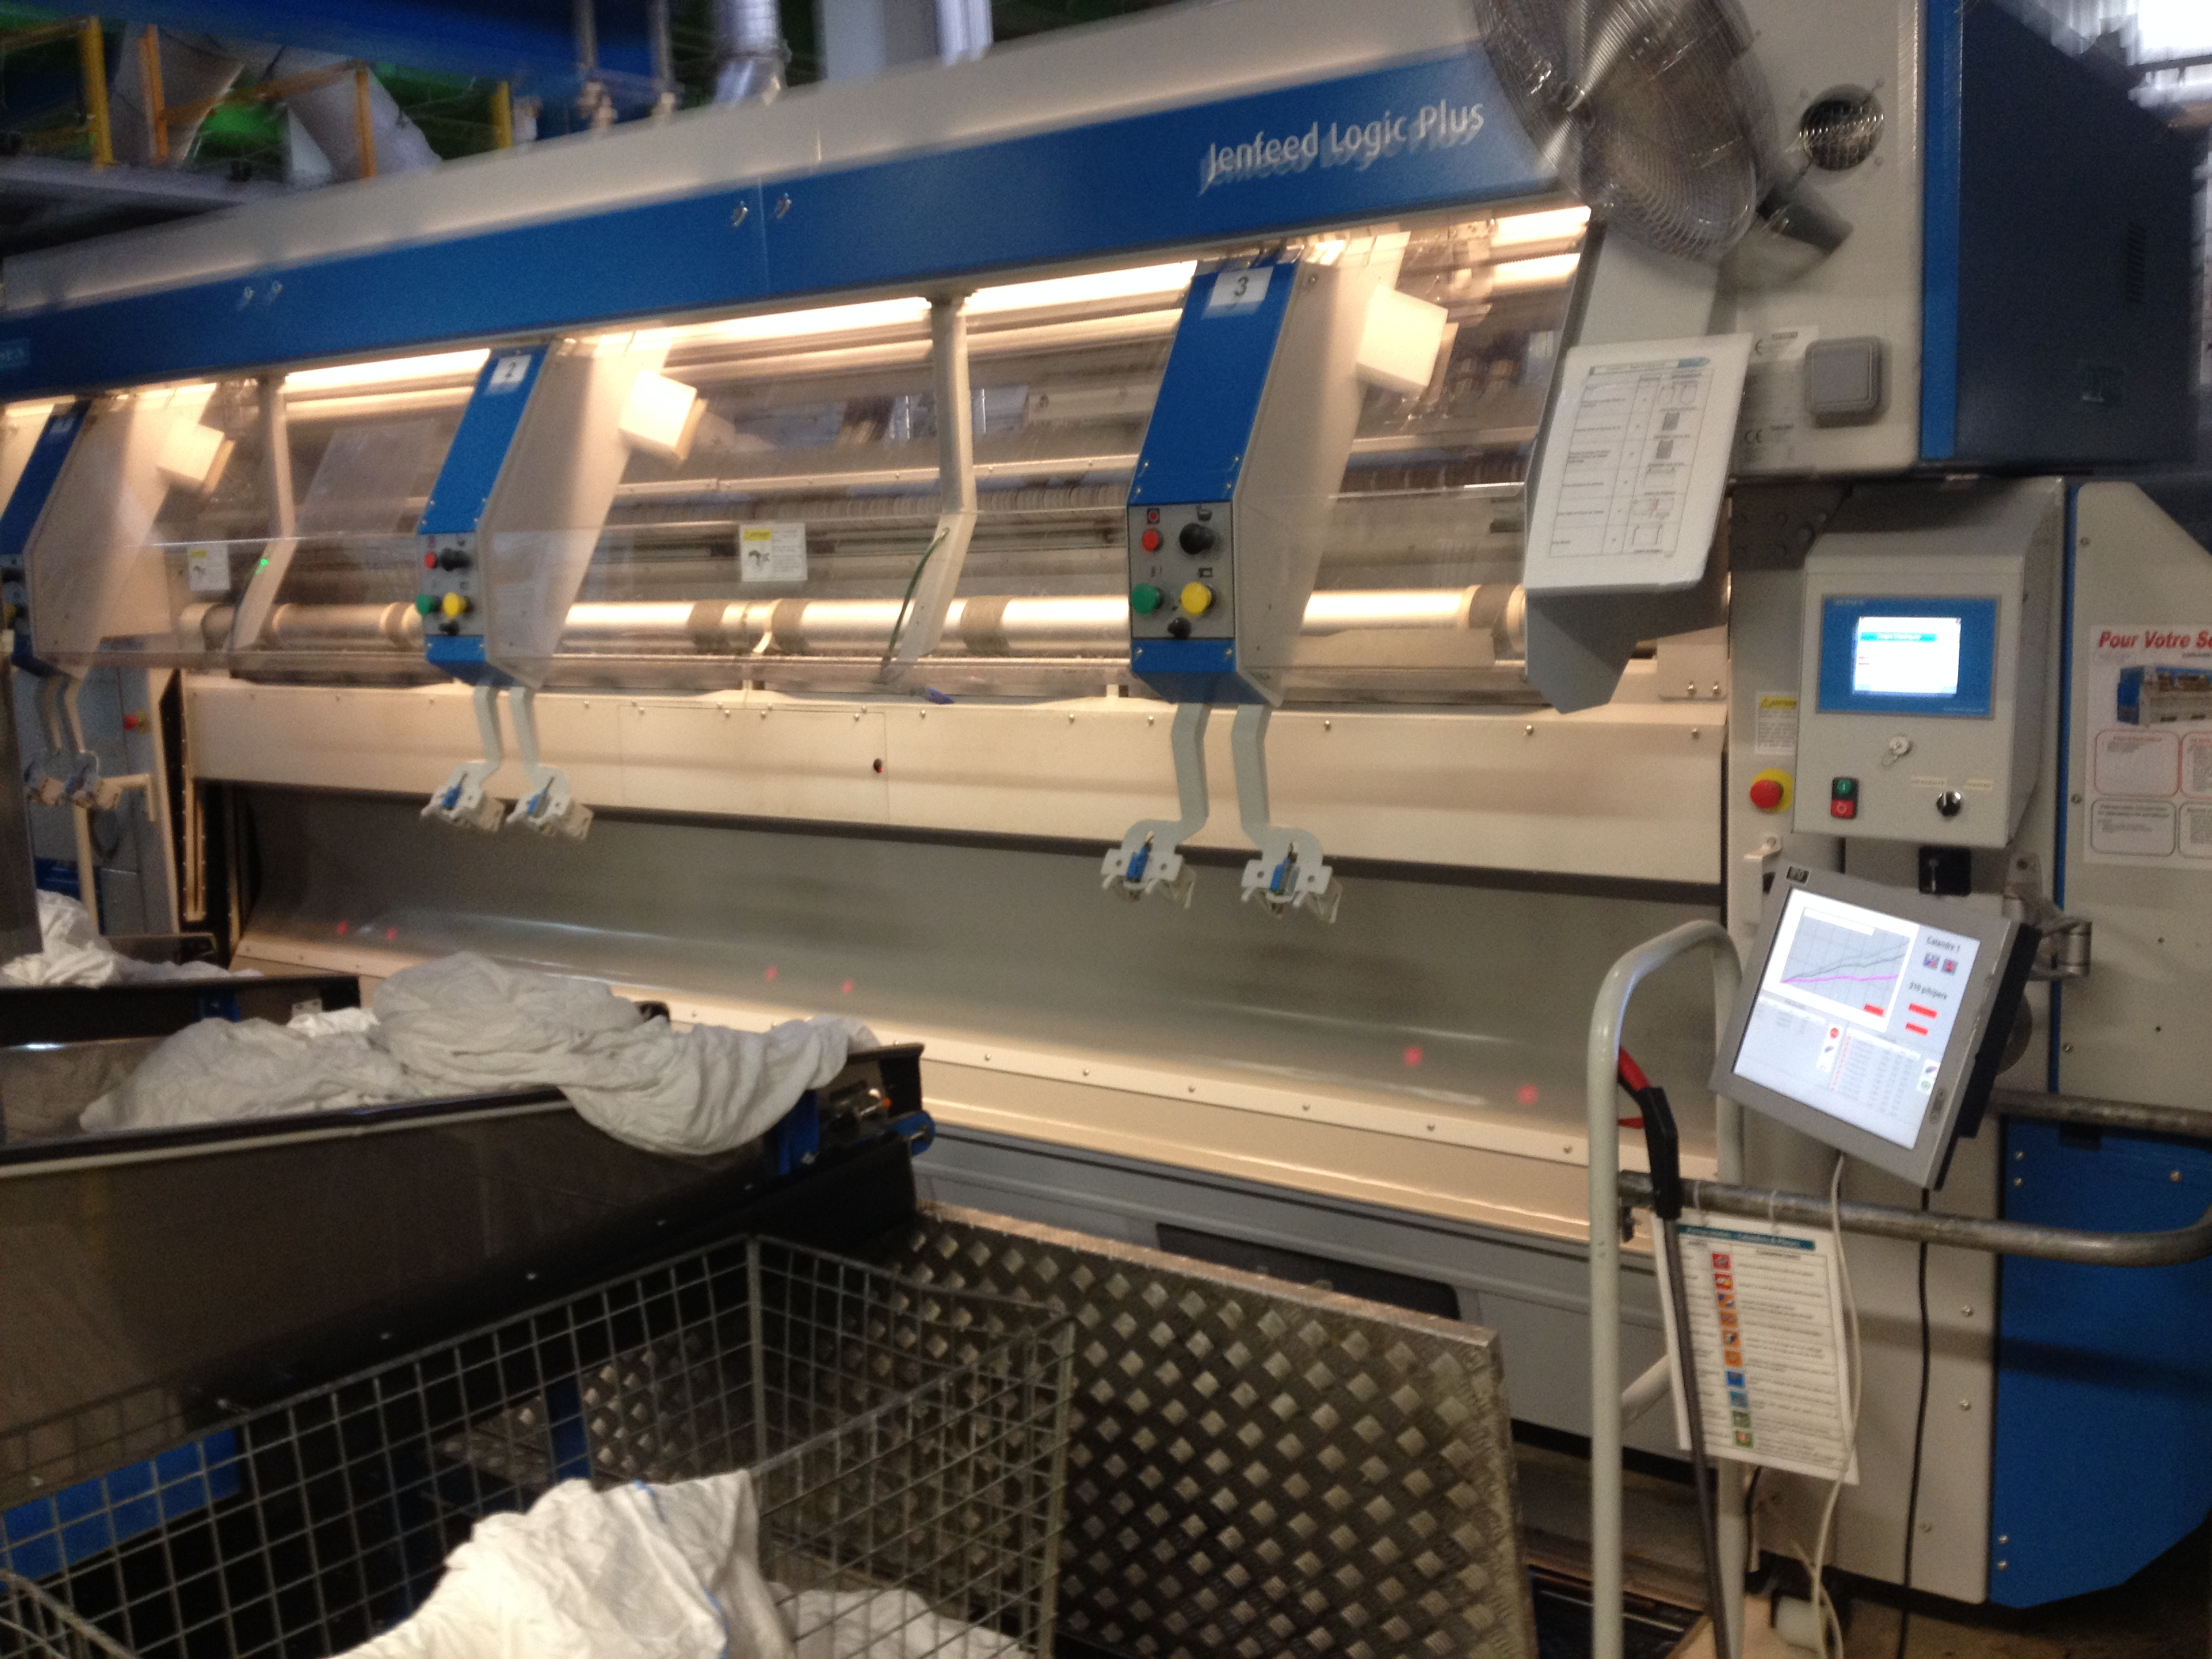
\includegraphics[scale= \rapportSubFigure]{images/calandre}
        \caption{Vu d'ensemble.}
        \label{fig:calandre}
    \end{subfigure}
    ~
    \begin{subfigure}{0.49\textwidth}
        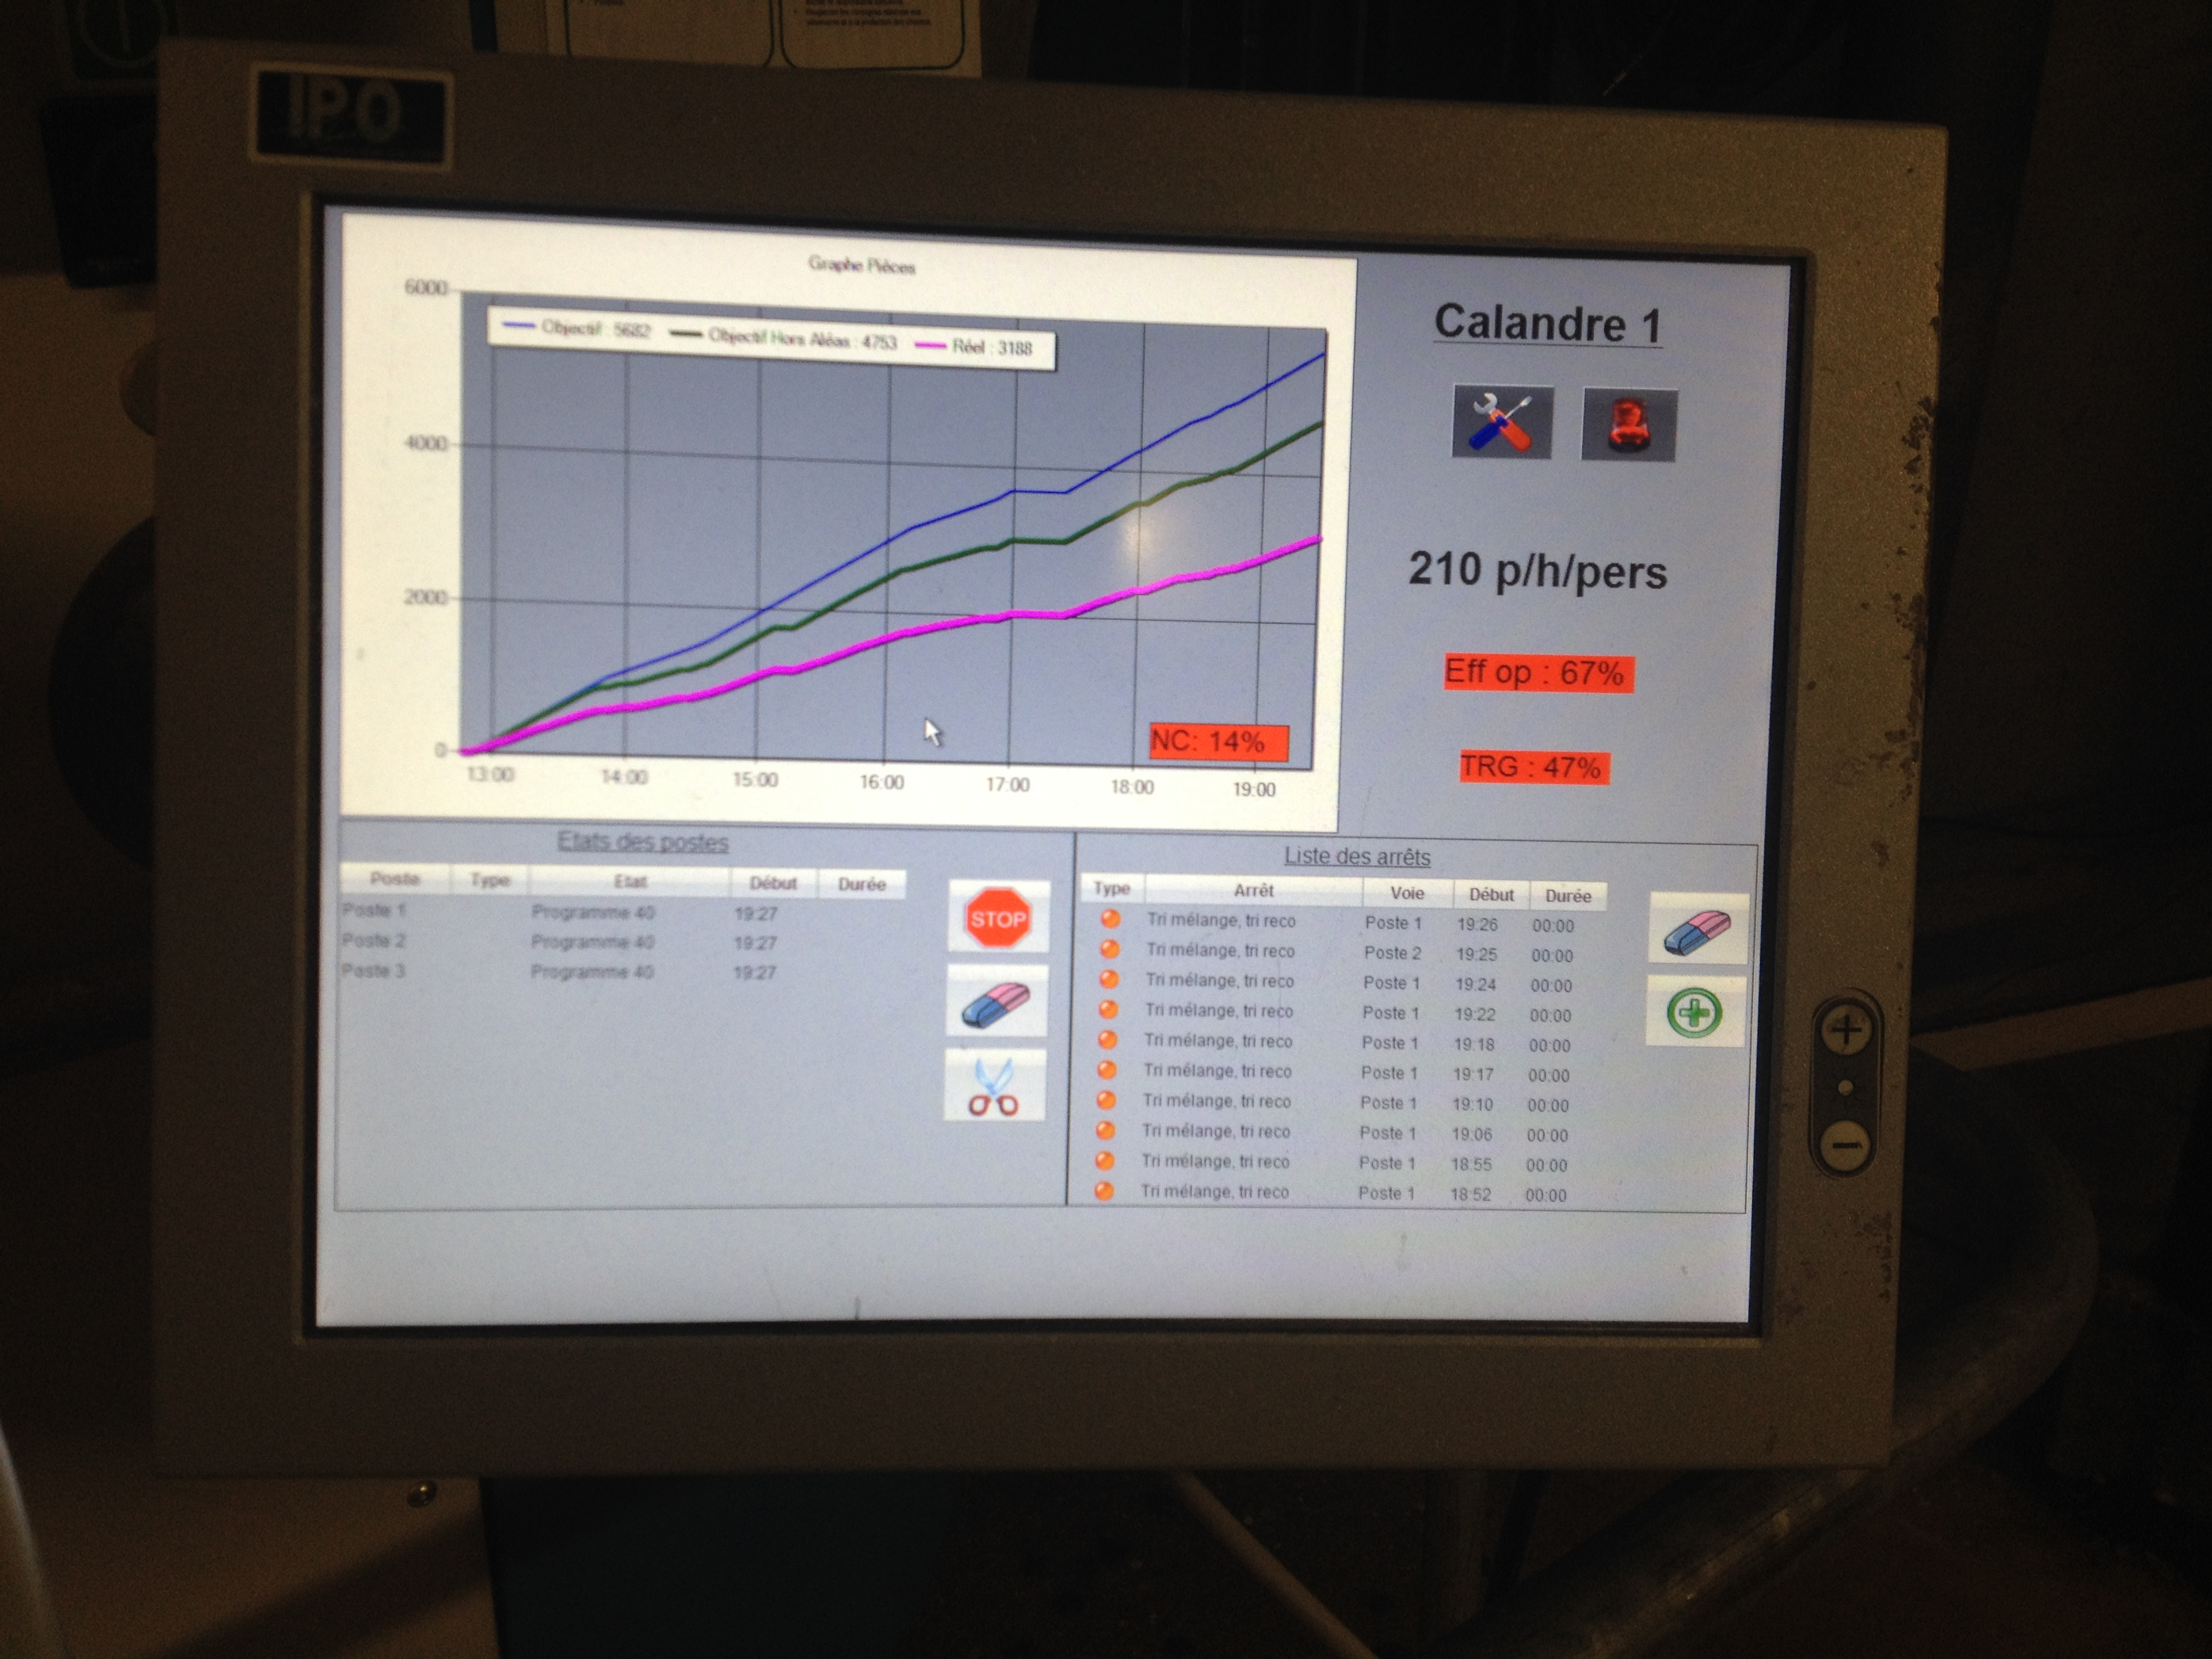
\includegraphics[scale= \rapportSubFigure]{images/calandre_controle}
        \caption{Ecran de contrôle de calandre.}
        \label{fig:ecran}
    \end{subfigure}
    
    \caption{Une calandre.}
\end{figure}
%
\FloatBarrier


\subsubsection{Préparation des Commandes}

La préparation des commandes étant la dérnière étape avant la livraison au
client, exige toujours l'attention de l'opérateur. Elle exige ainsi surtout de
la responsabilité et de l'engagement. Les sections suivantes visent à la
détailler.

\paragraph{Les Sacs}

La dernière étape (avant le client) est la préparation des sacs. Son contenu est
déterminé à partir d'une fiche, comme celle en vert de la figure
\ref{fig:fiche}. On peut y voir toutes les informations du client, comme nom et
adresse, son code (ici, 604966), la date de livraison (dans notre cas le lundi
15 septembre) et aussi ce qu'on doit mettre dans le respectif sac. Enfin, le
numéro de la tournée - voir section \ref{sec:tournee} - indique où l'on doit
amener le chariot (figure \ref{fig:sacs}) pour qu'il soit bien livré.

\vspace{12pt}

Après avoir fini chaque client, il faut bien prendre note de la
quantité des sacs faits. Cela est réalisé à l'aide de la feuille de clients,
répresentée également à la figure \ref{fig:fiche}.

\FloatBarrier
%
\begin{figure}[h]
    \begin{subfigure}{0.49\textwidth}
        \centering
        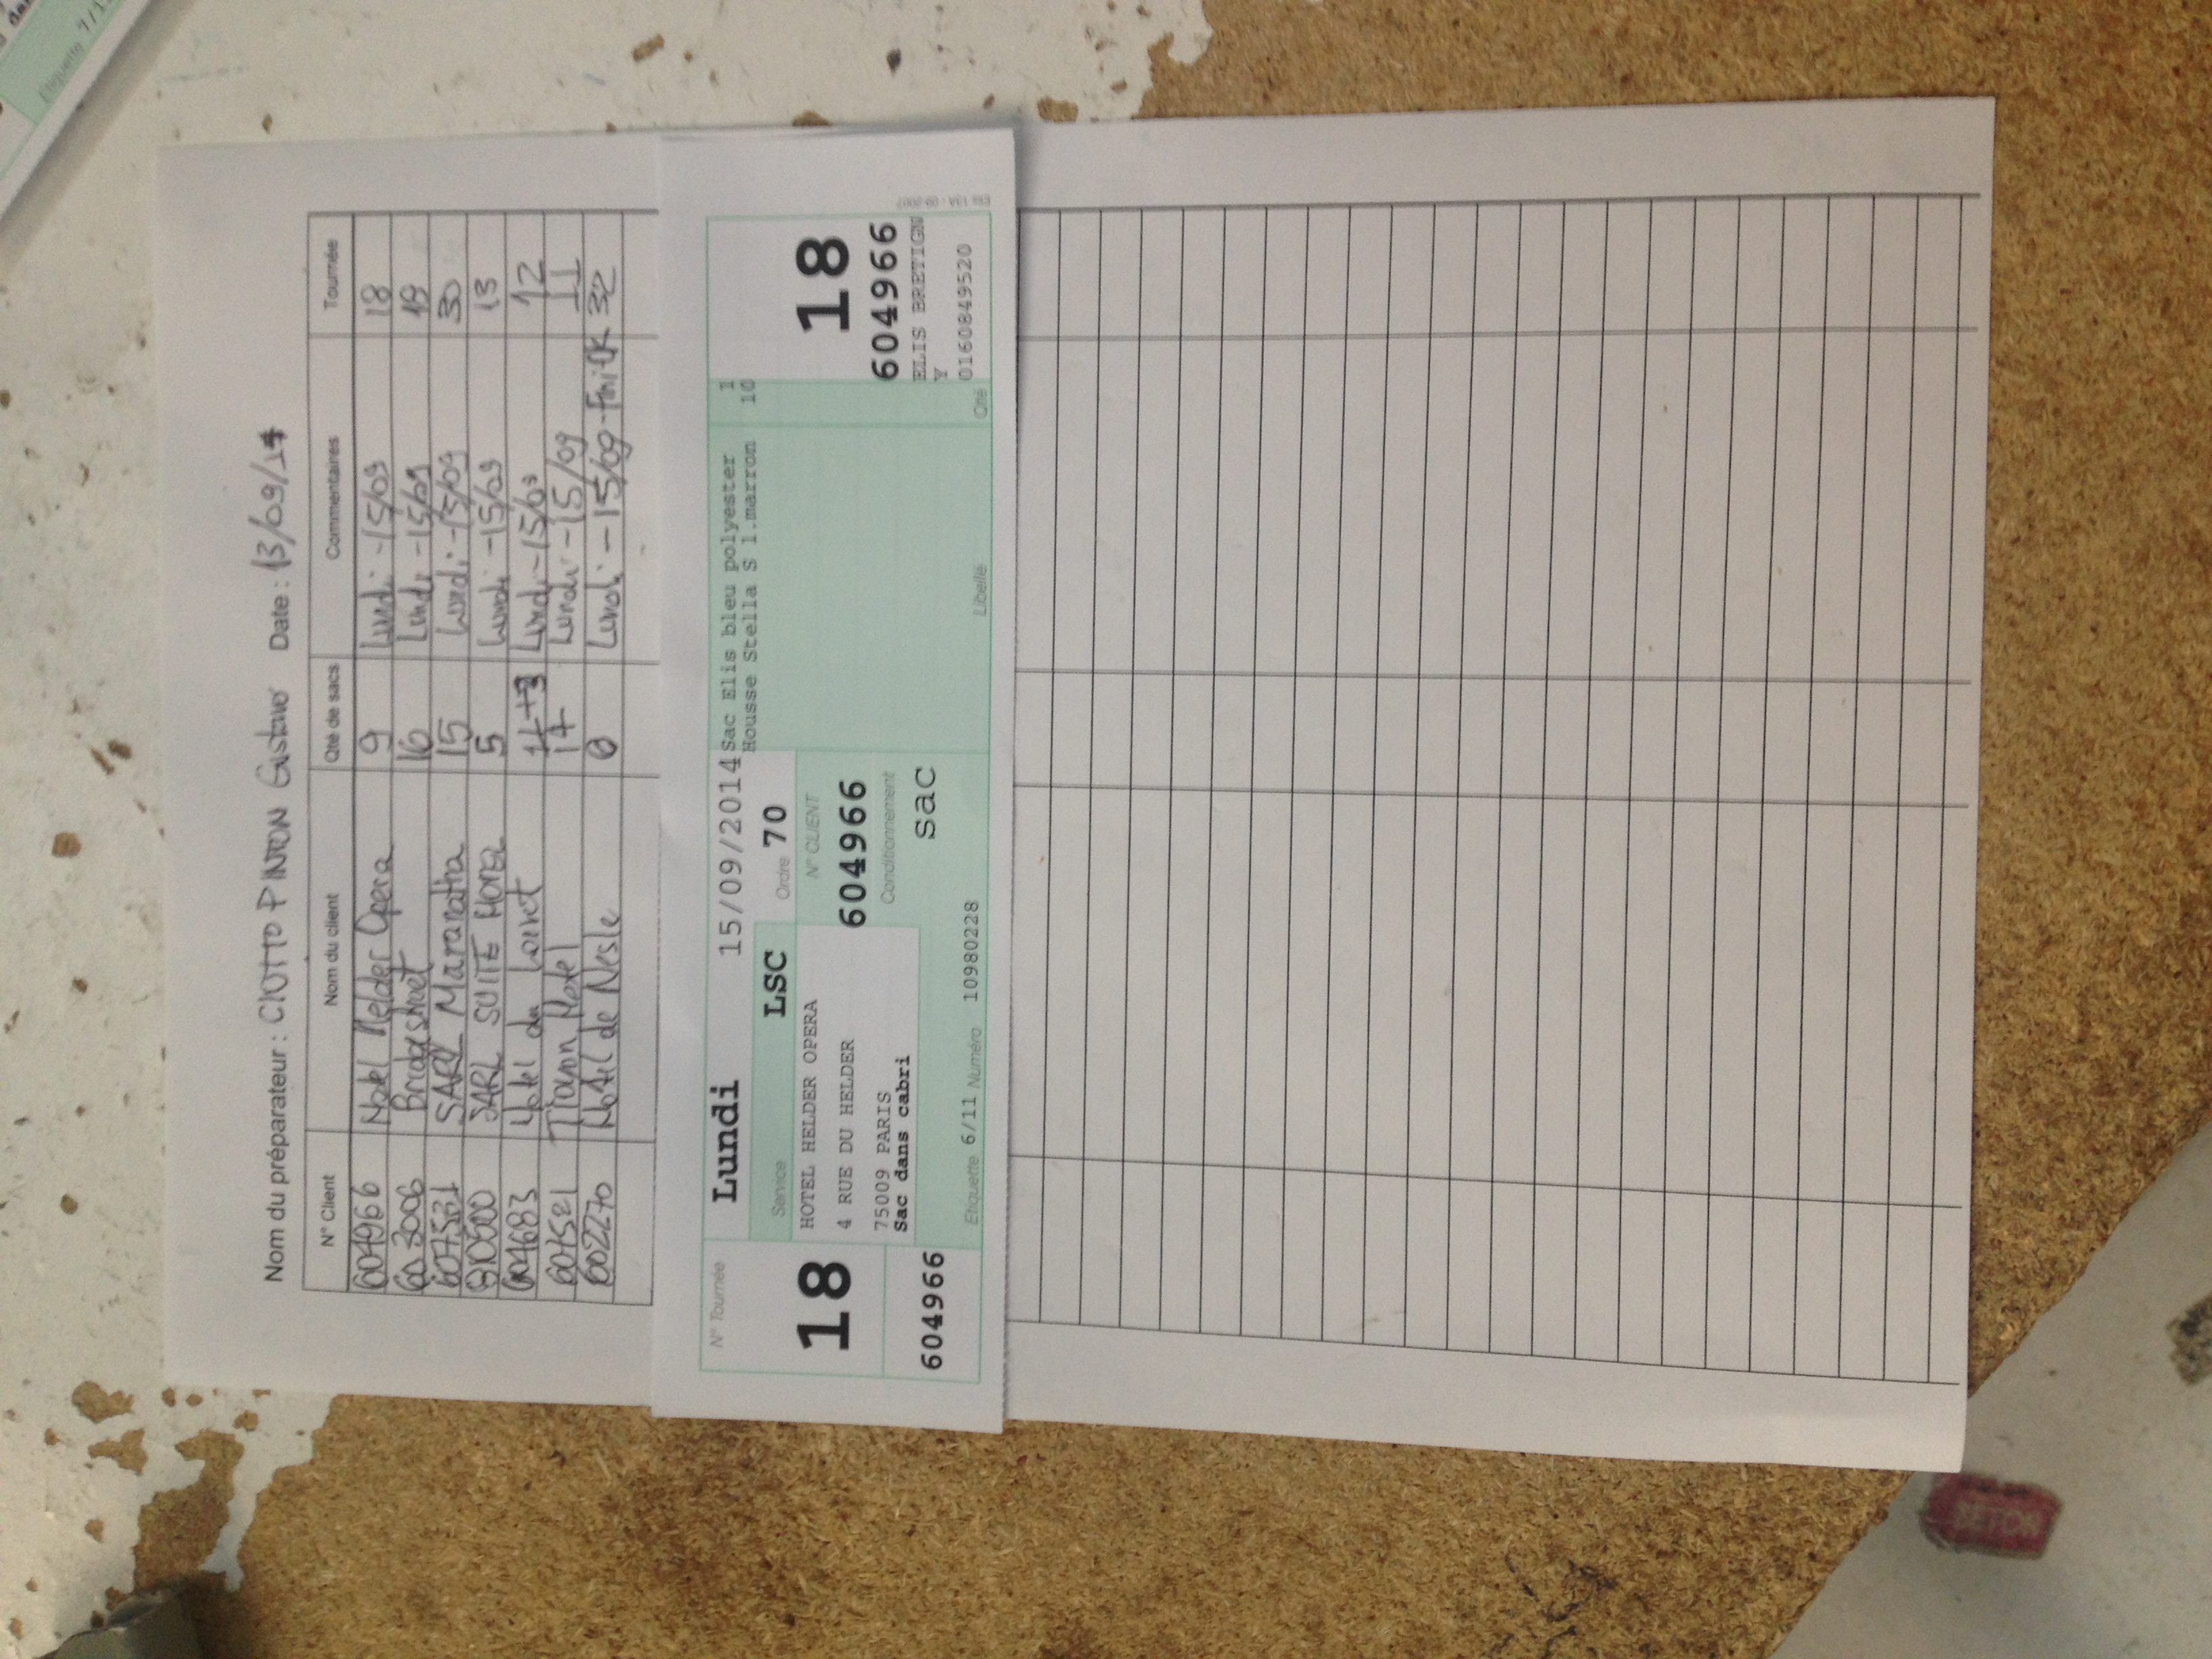
\includegraphics[angle=-90,scale= \rapportFigure]{images/fiche_sacs}
        \caption{Le feuille de clients et une fiche de préparation.}
        \label{fig:fiche}
    \end{subfigure}
    ~
    \begin{subfigure}{0.49\textwidth}
        \centering
        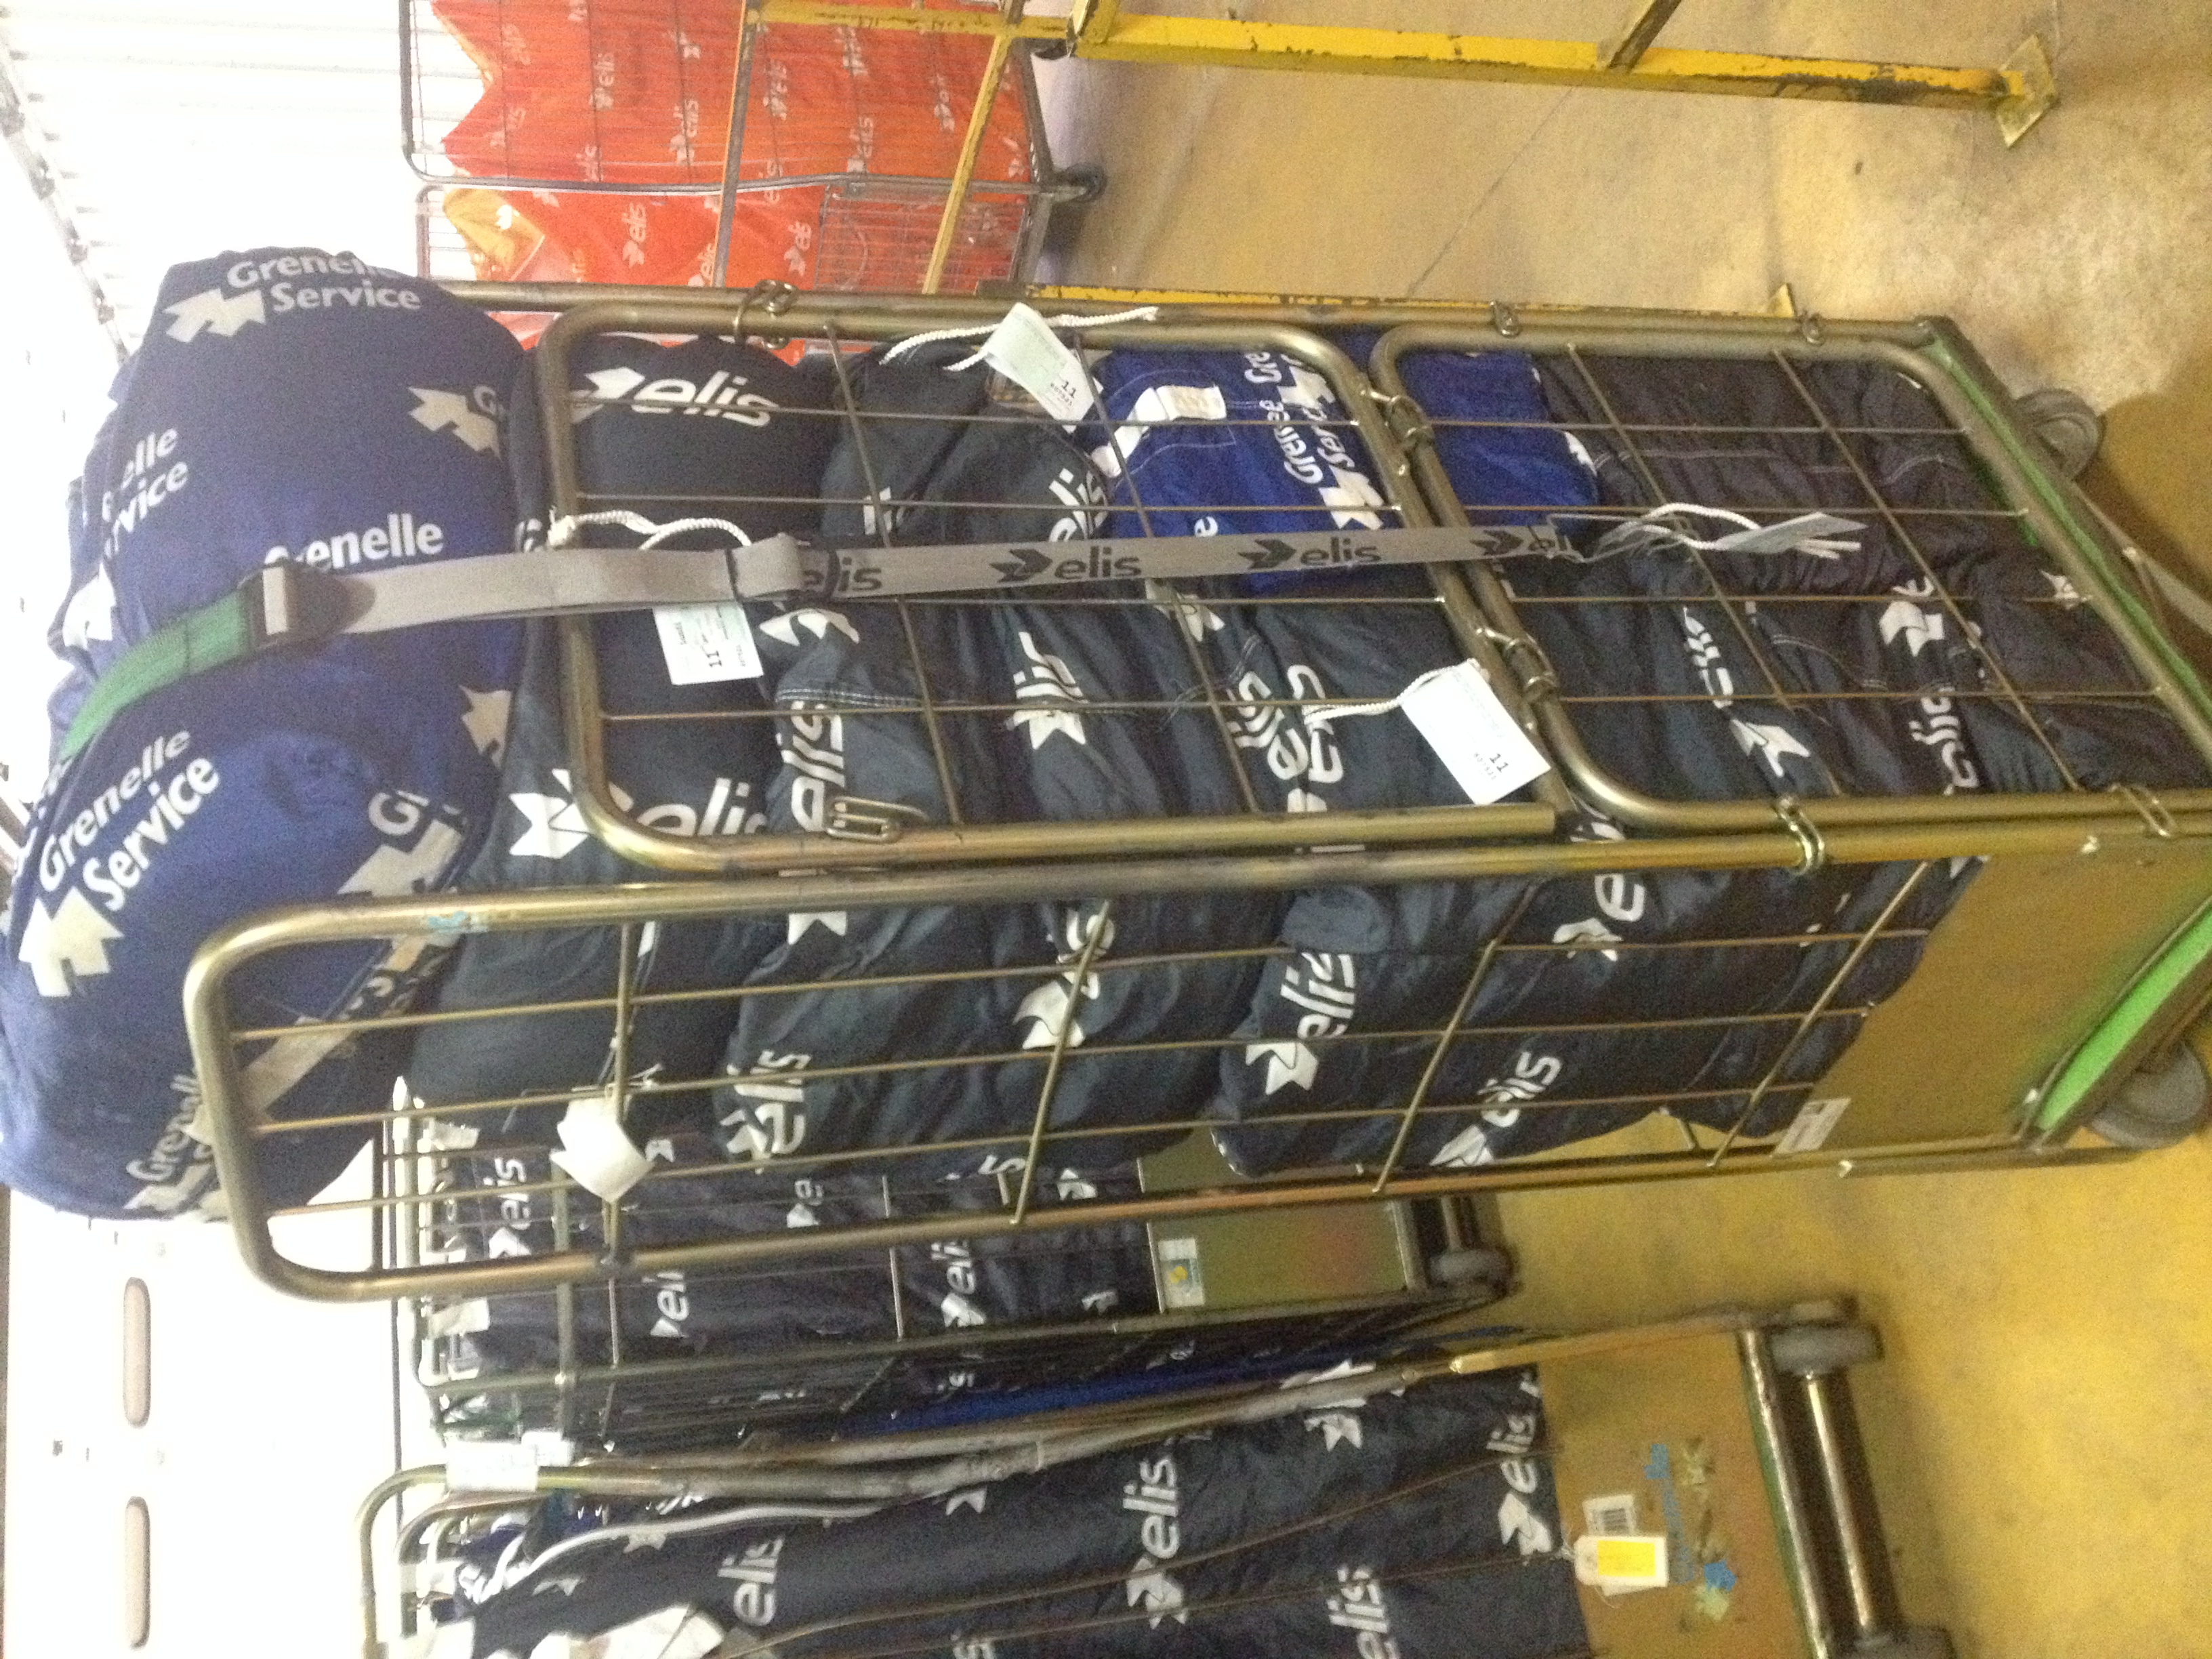
\includegraphics[angle=-90,scale= \rapportFigure]{images/chariot}
        \caption{Chariot prêt à être livré.}
        \label{fig:sacs}
    \end{subfigure}
    
    \caption{Opération à l'expédition.}
\end{figure}
%
\FloatBarrier

\paragraph{Pousser les Chariots}
\label{sec:tournee}

Les produits d'un client doivent alors être amenés à sa respective tournée
après la fiche (figure \ref{fig:fiche}). C'est la tâche attribuée à
l'opérateur responsable pour pousser les chariots. C'est à lui de connaître où
sont situées les tournées et de veiller à l'organisation des chariots sur toutes
les quais. Les figures \ref{fig:exp} et \ref{fig:tournee} montrent
respectivement la vue générale de l'expédition et une tournée en détail.


%
\begin{figure}[h]
    \begin{subfigure}{0.53\textwidth}
        \centering
        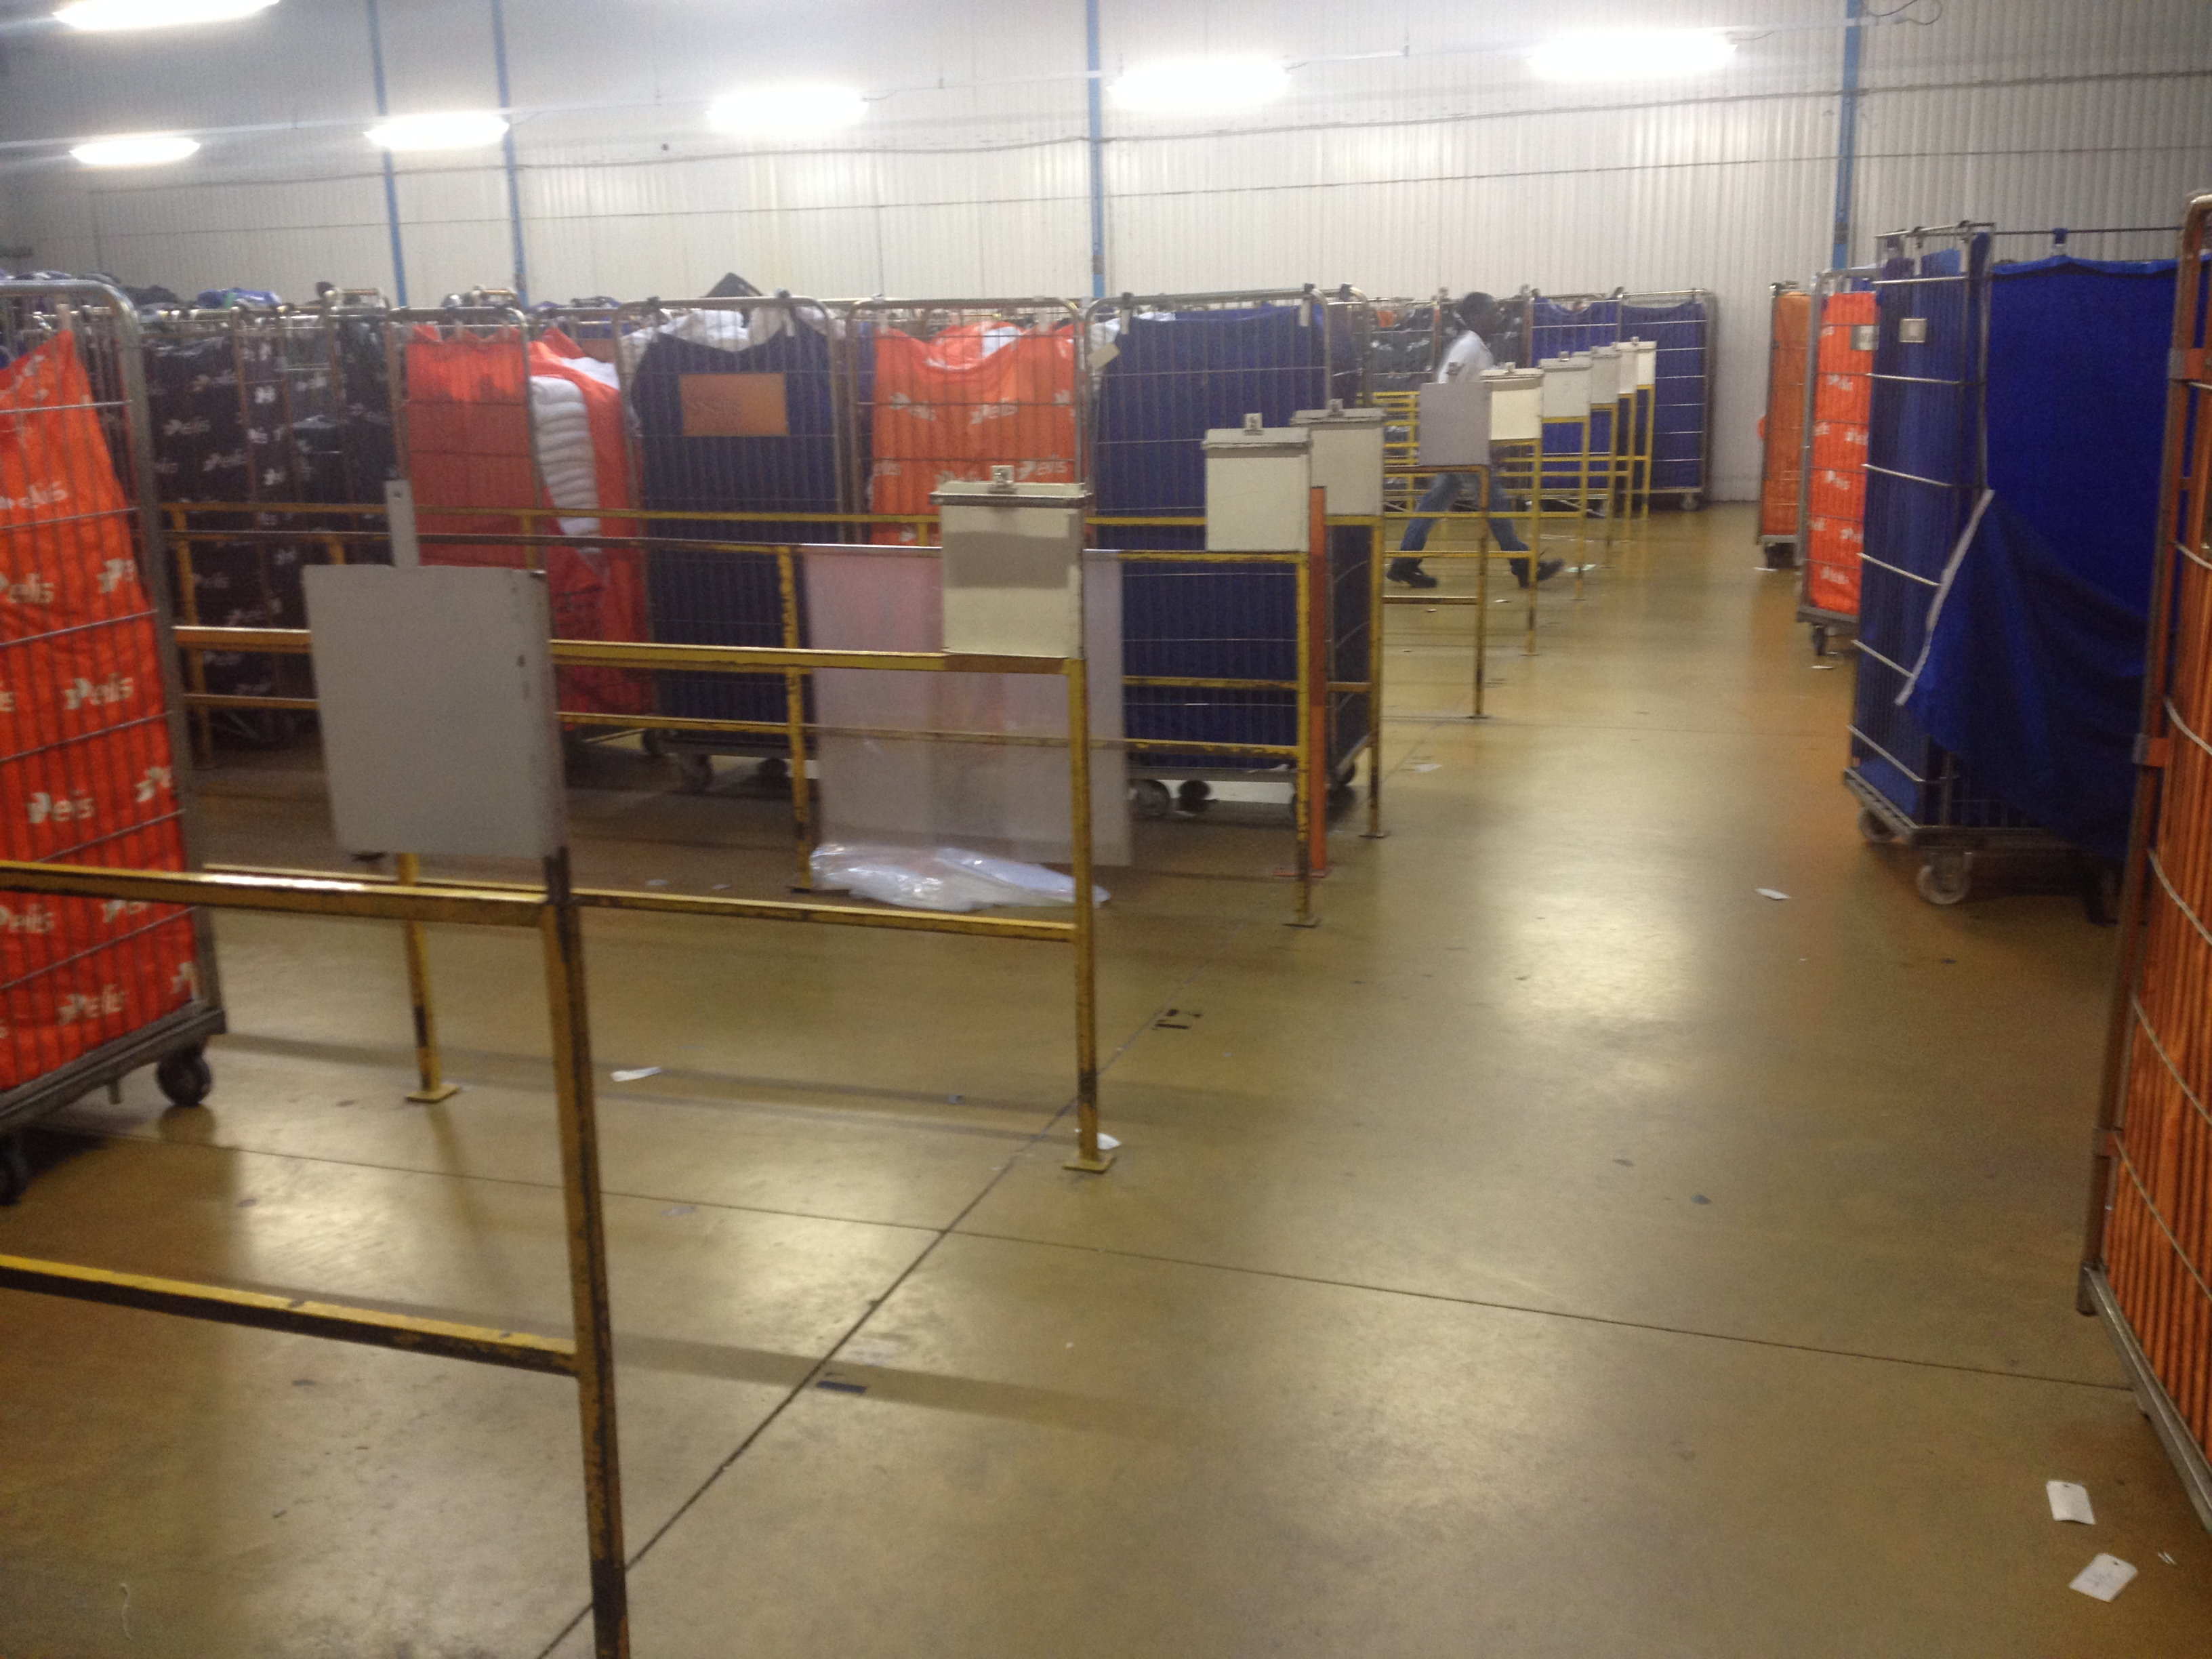
\includegraphics[scale= 0.078]{images/expedition}
        \caption{Vue de l'expédition.}
        \label{fig:exp}
    \end{subfigure}
    ~
    \begin{subfigure}{0.44\textwidth}
        \centering
        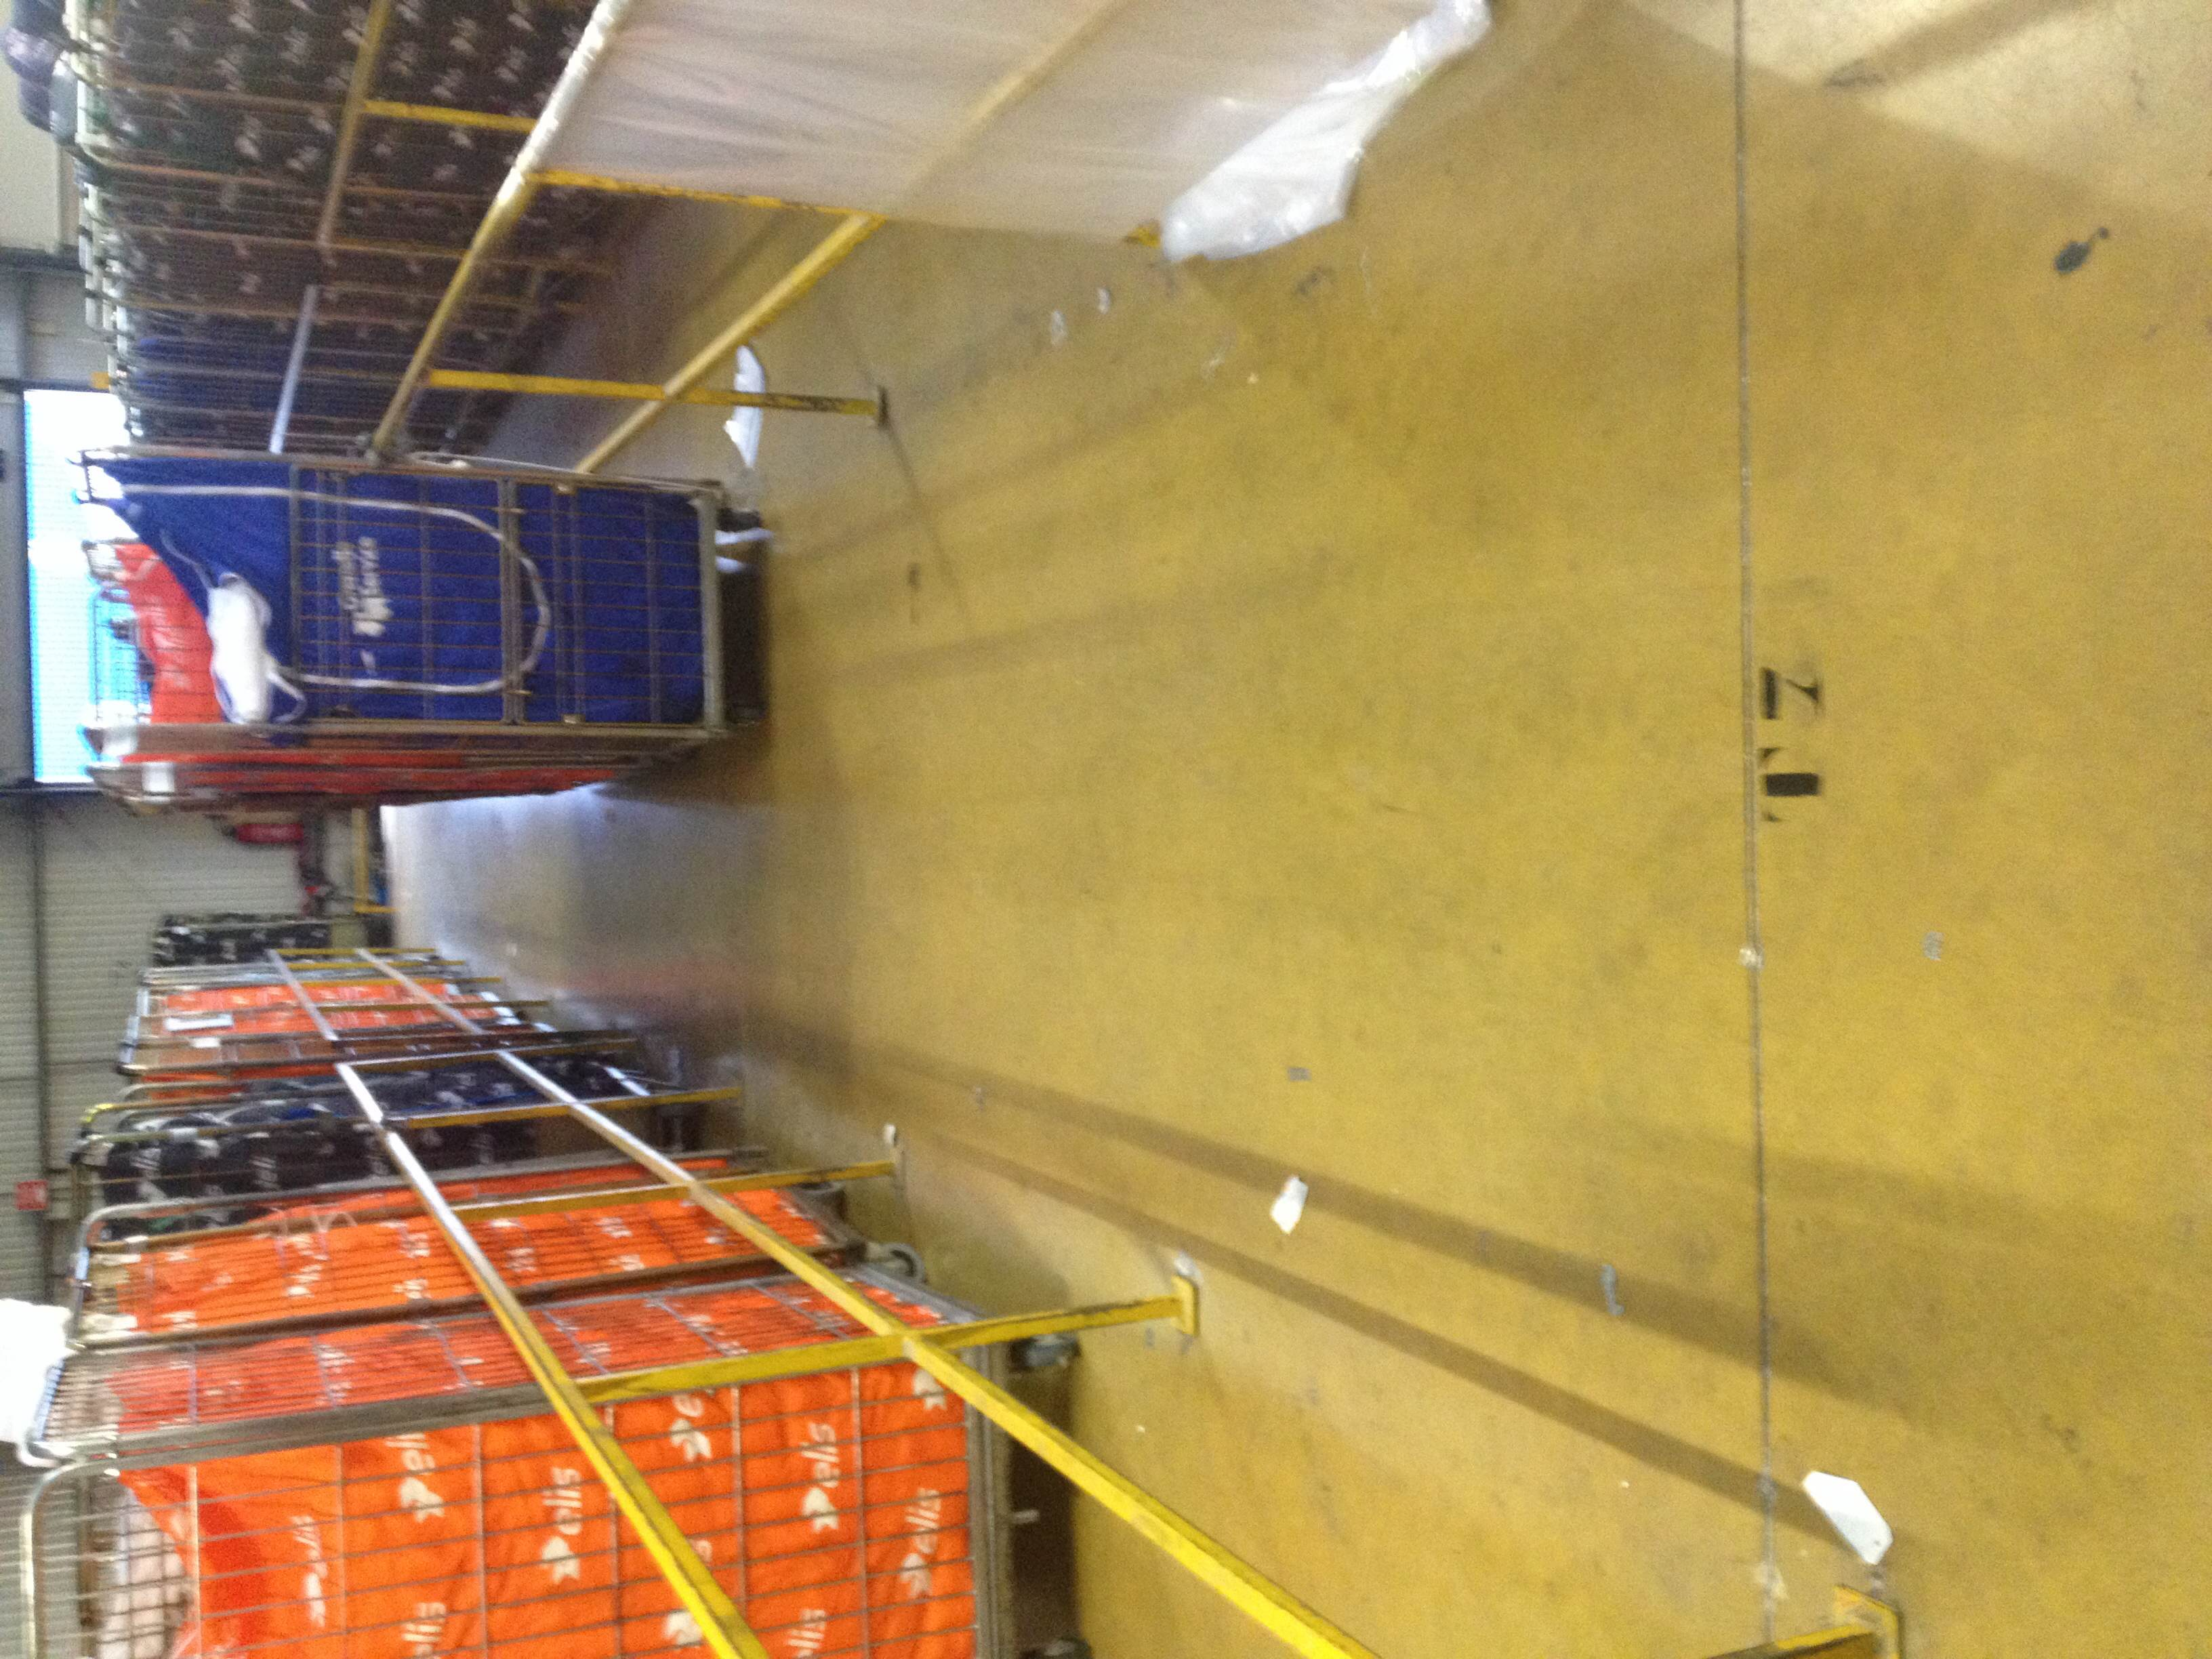
\includegraphics[angle=-90,scale= \rapportFigure]{images/tournee}
        \caption{La tournée où les chariots prêts à livraison sont ramenés.}
        \label{fig:tournee}
    \end{subfigure}
    
    \caption{L'expédition.}
\end{figure}
%

\subsubsection{Carré Revisage}

Le \og carré revisage \fg~ consiste à trier des petites éponges de
format carré en piles de 25, comme sur la figure \ref{fig:carre}. Il faut
remarquer aussi que l'opérateur doit être toujours vigilant par rapport aux
pièces contenant des taches ou ceux qui sont déchirés.

\FloatBarrier

\begin{figure}[h]
    \centering 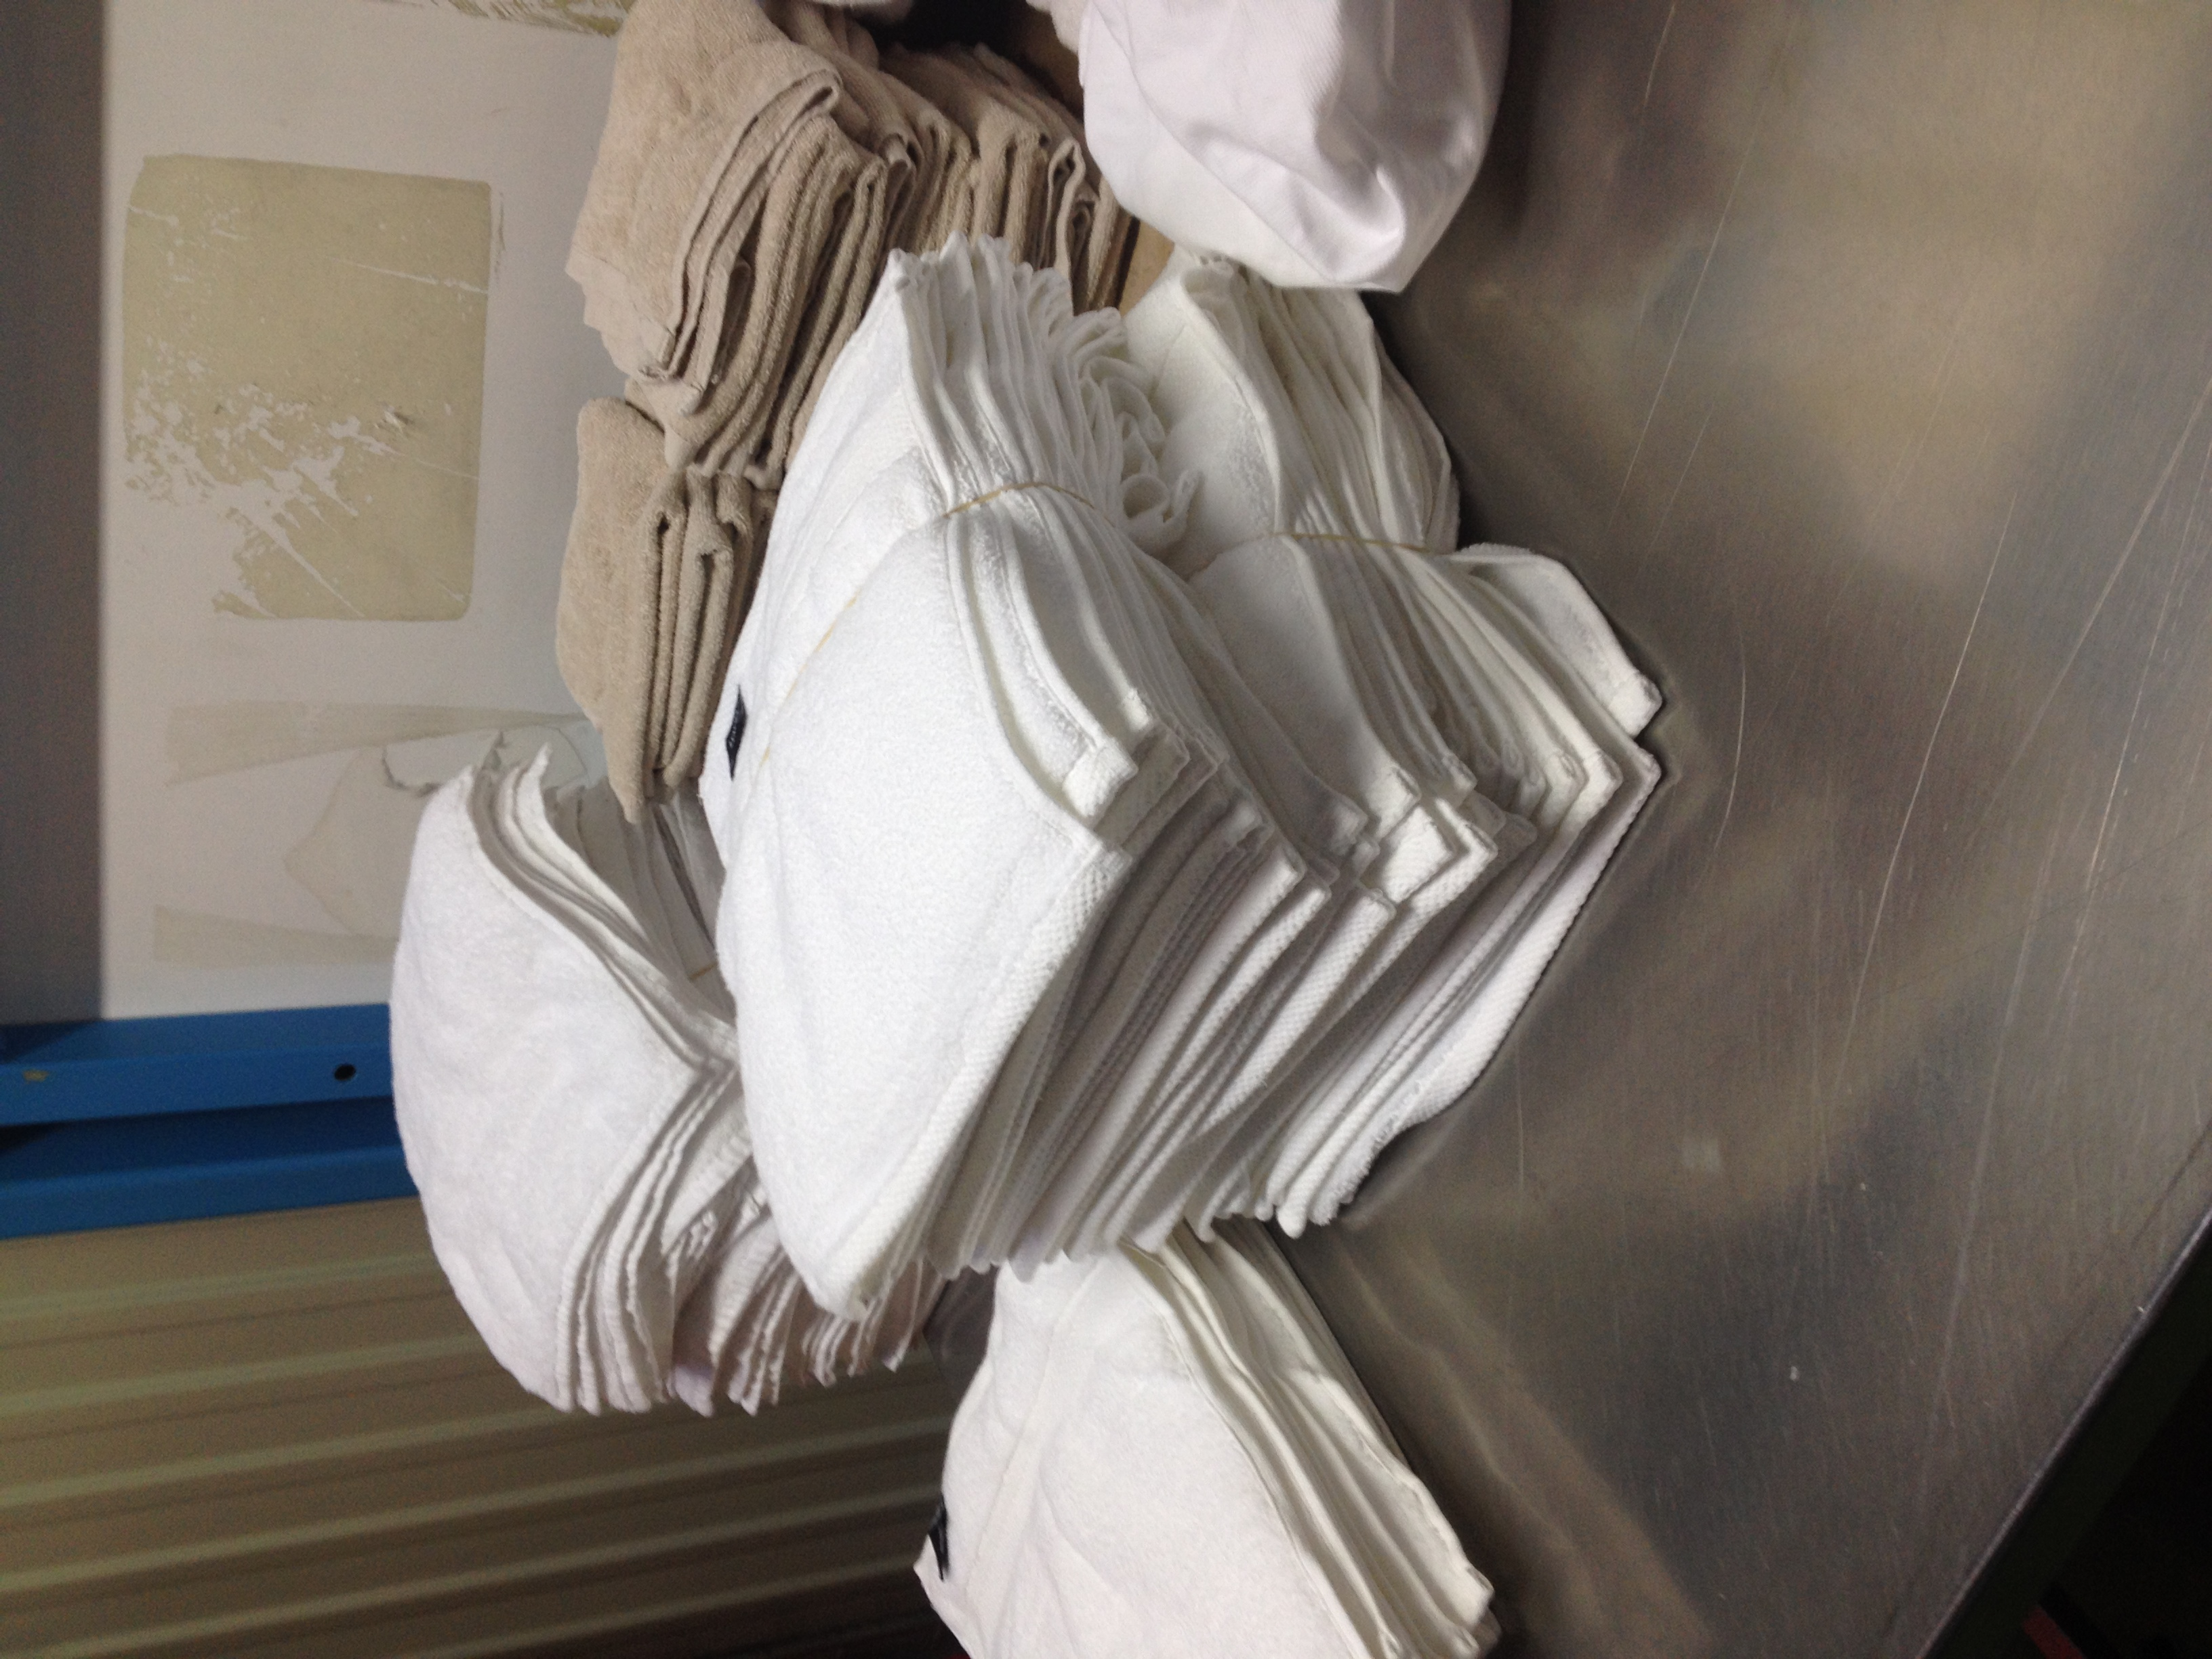
\includegraphics[angle = -90, scale=
    \rapportFigure]{images/carre}
    \caption{Piles avec 25 de pièces carrées.}
    \label{fig:carre}
\end{figure}
\FloatBarrier


\subsubsection{Le RECO}

L'activité appelée \og RECO \fg ~consiste au triage du linge qui, pour
certaines raisons, a été mal plié par les calandres ou a été rejeté par les
opérateurs à cause des taches ou déchirures. Le responsable doit alors bien
identifier sa catégorie et le placer dans le bon chariot. La disposition de
chariots et les étiquettes utilisées avec le but d'aider l'identification des
caractéristiques sont montrées dans les figure \ref{fig:reco} et
\ref{fig:etiquette_reco}.

\FloatBarrier
%
\begin{figure}[h]
    \begin{subfigure}{0.49\textwidth}
        \centering
        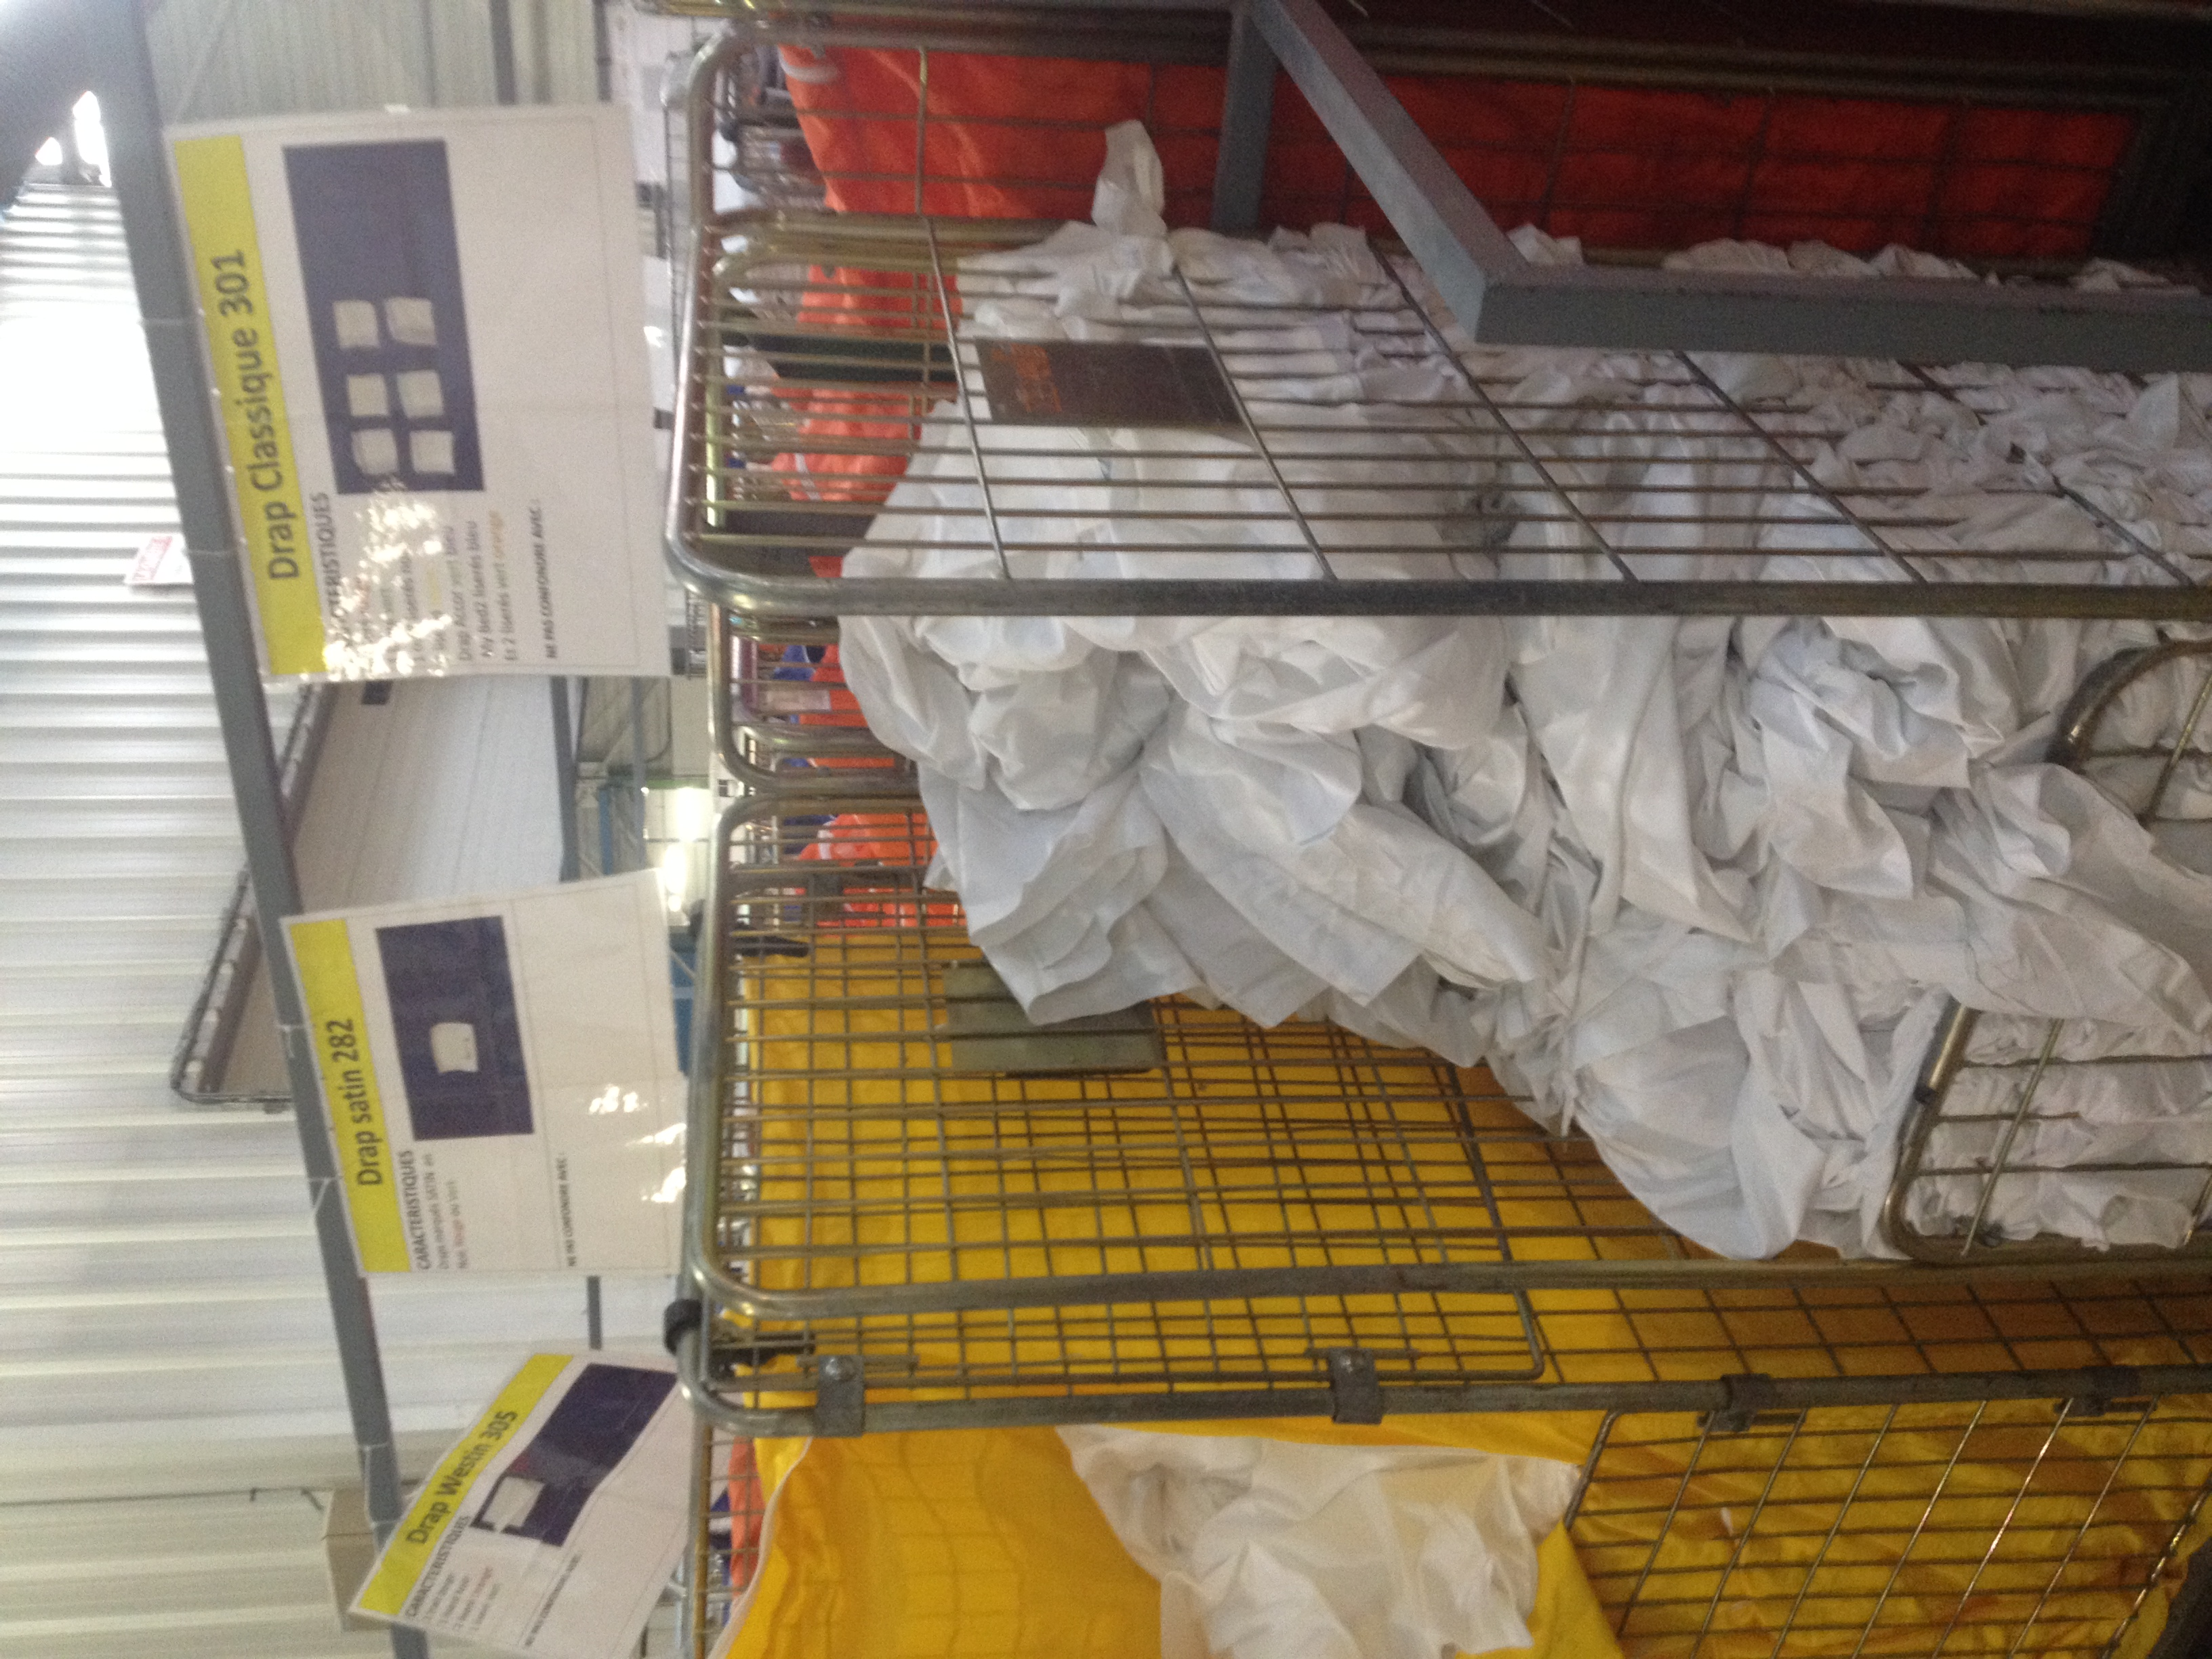
\includegraphics[angle=-90, scale= \rapportFigure]{images/reco}
        \caption{Disposition physique des chariots destinés au \og reco \fg.}
        \label{fig:reco}
    \end{subfigure}
    ~
    \begin{subfigure}{0.49\textwidth}
        \centering
        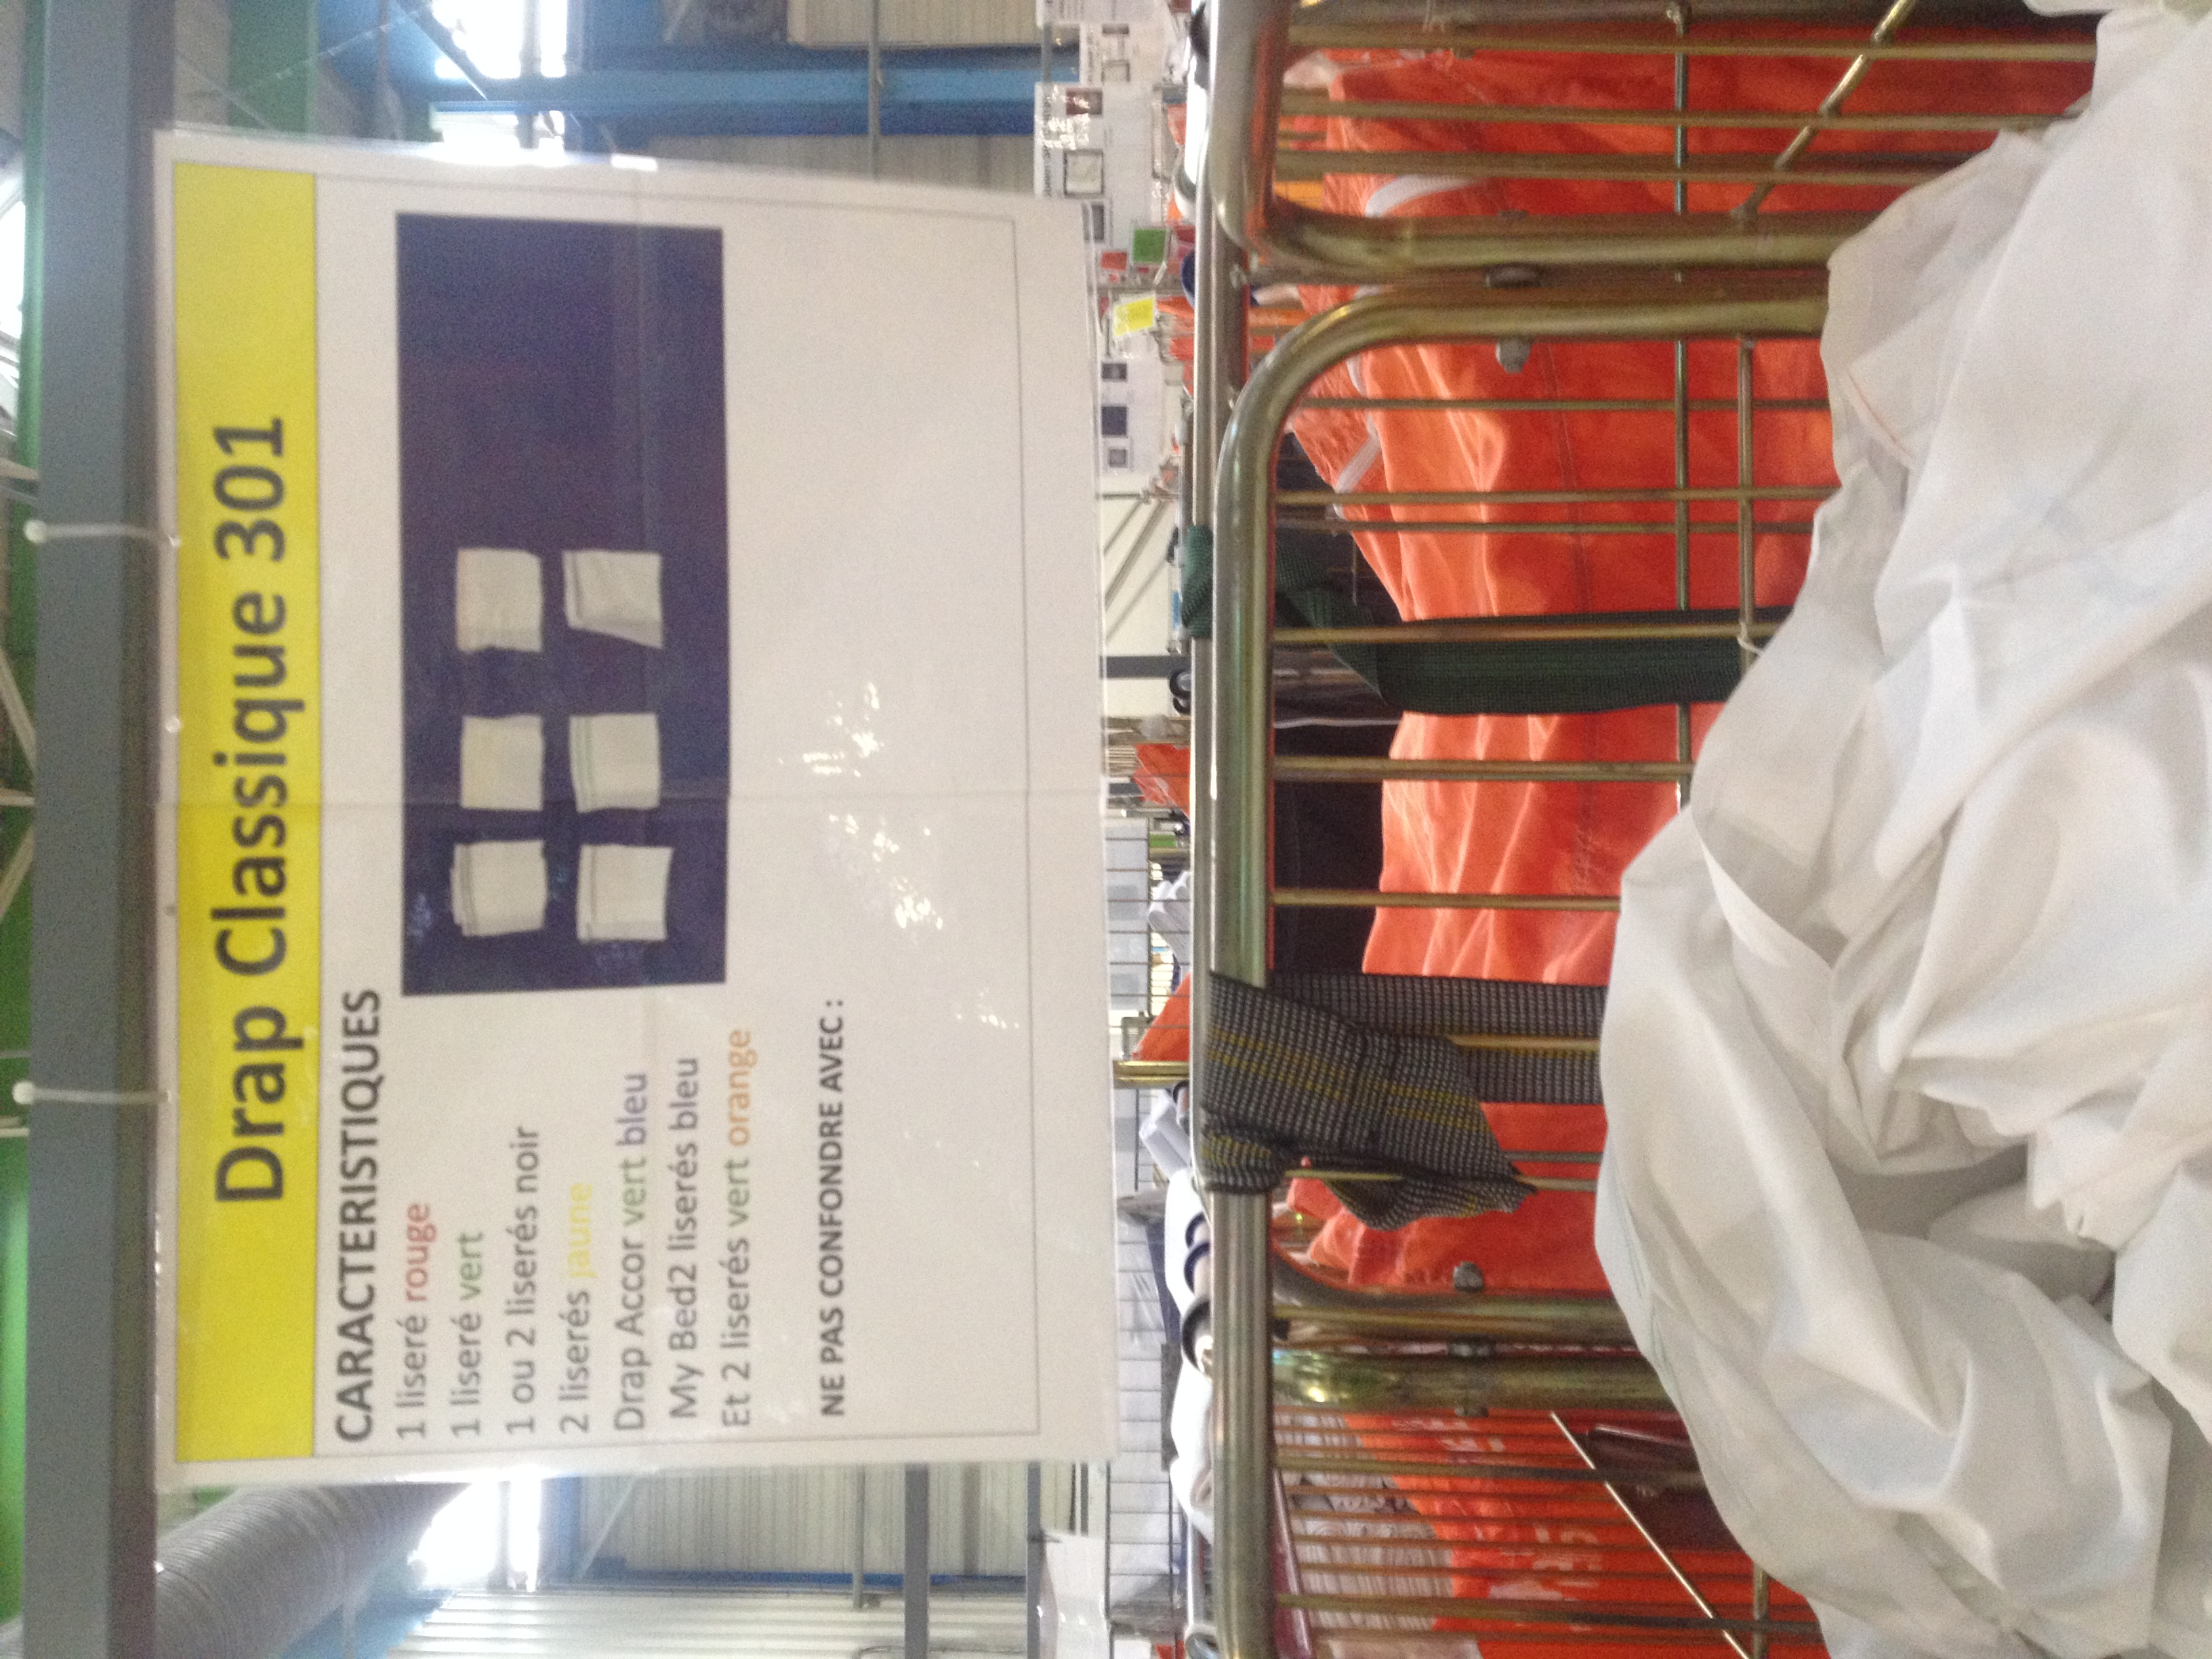
\includegraphics[angle=-90,scale= \rapportFigure]{images/reco_fiche}
        \caption{Etiquette d'identification.}
        \label{fig:etiquette_reco}
    \end{subfigure}
    
    \caption{Opération au RECO.}
\end{figure}
%
\FloatBarrier

\newpage 

\subsection{Restauration}

La restauration s'engage à préparer des taies, sous-taies et nappes.

\subsubsection{Management des passes}

L'opérateur désigné à cette activité décide ce qui sera engagé sur
les machines, ayant ainsi une tâche de très haute responsabilité. Tout au début,
il reçoit une feuille contenant les besoins du jour et ce qui doit sortir en
priorité. A la figure \ref{fig:management}, est montré l'écran du logiciel qui
controlê les conteneurs de linge, répresentés chacun par un petit cercle
coloré. Ensuite, sur le coin inférieur à droite de l'image il y a une séquence
de conteneurs, appelée tunnel, d'où viennent des nouveaux conteneurs avec du linge
trié précédemment au contrôle entrée. Avant d'être prêts à l'engagement, le
linge de chaque conteneur doit passer par une presse mécanique et par un
sechoir. Le choix de cette dernière dépend de l'opérateur, qui peut choisir une
parmi les six disponibles. On remarque aussi dans le coin inférieur à gauche
qu'il y a douze places disponibles à la réserve de linge ou à la "man\oe uvre"
des conteneurs.

\FloatBarrier

%
\begin{figure}[h]
    \centering
    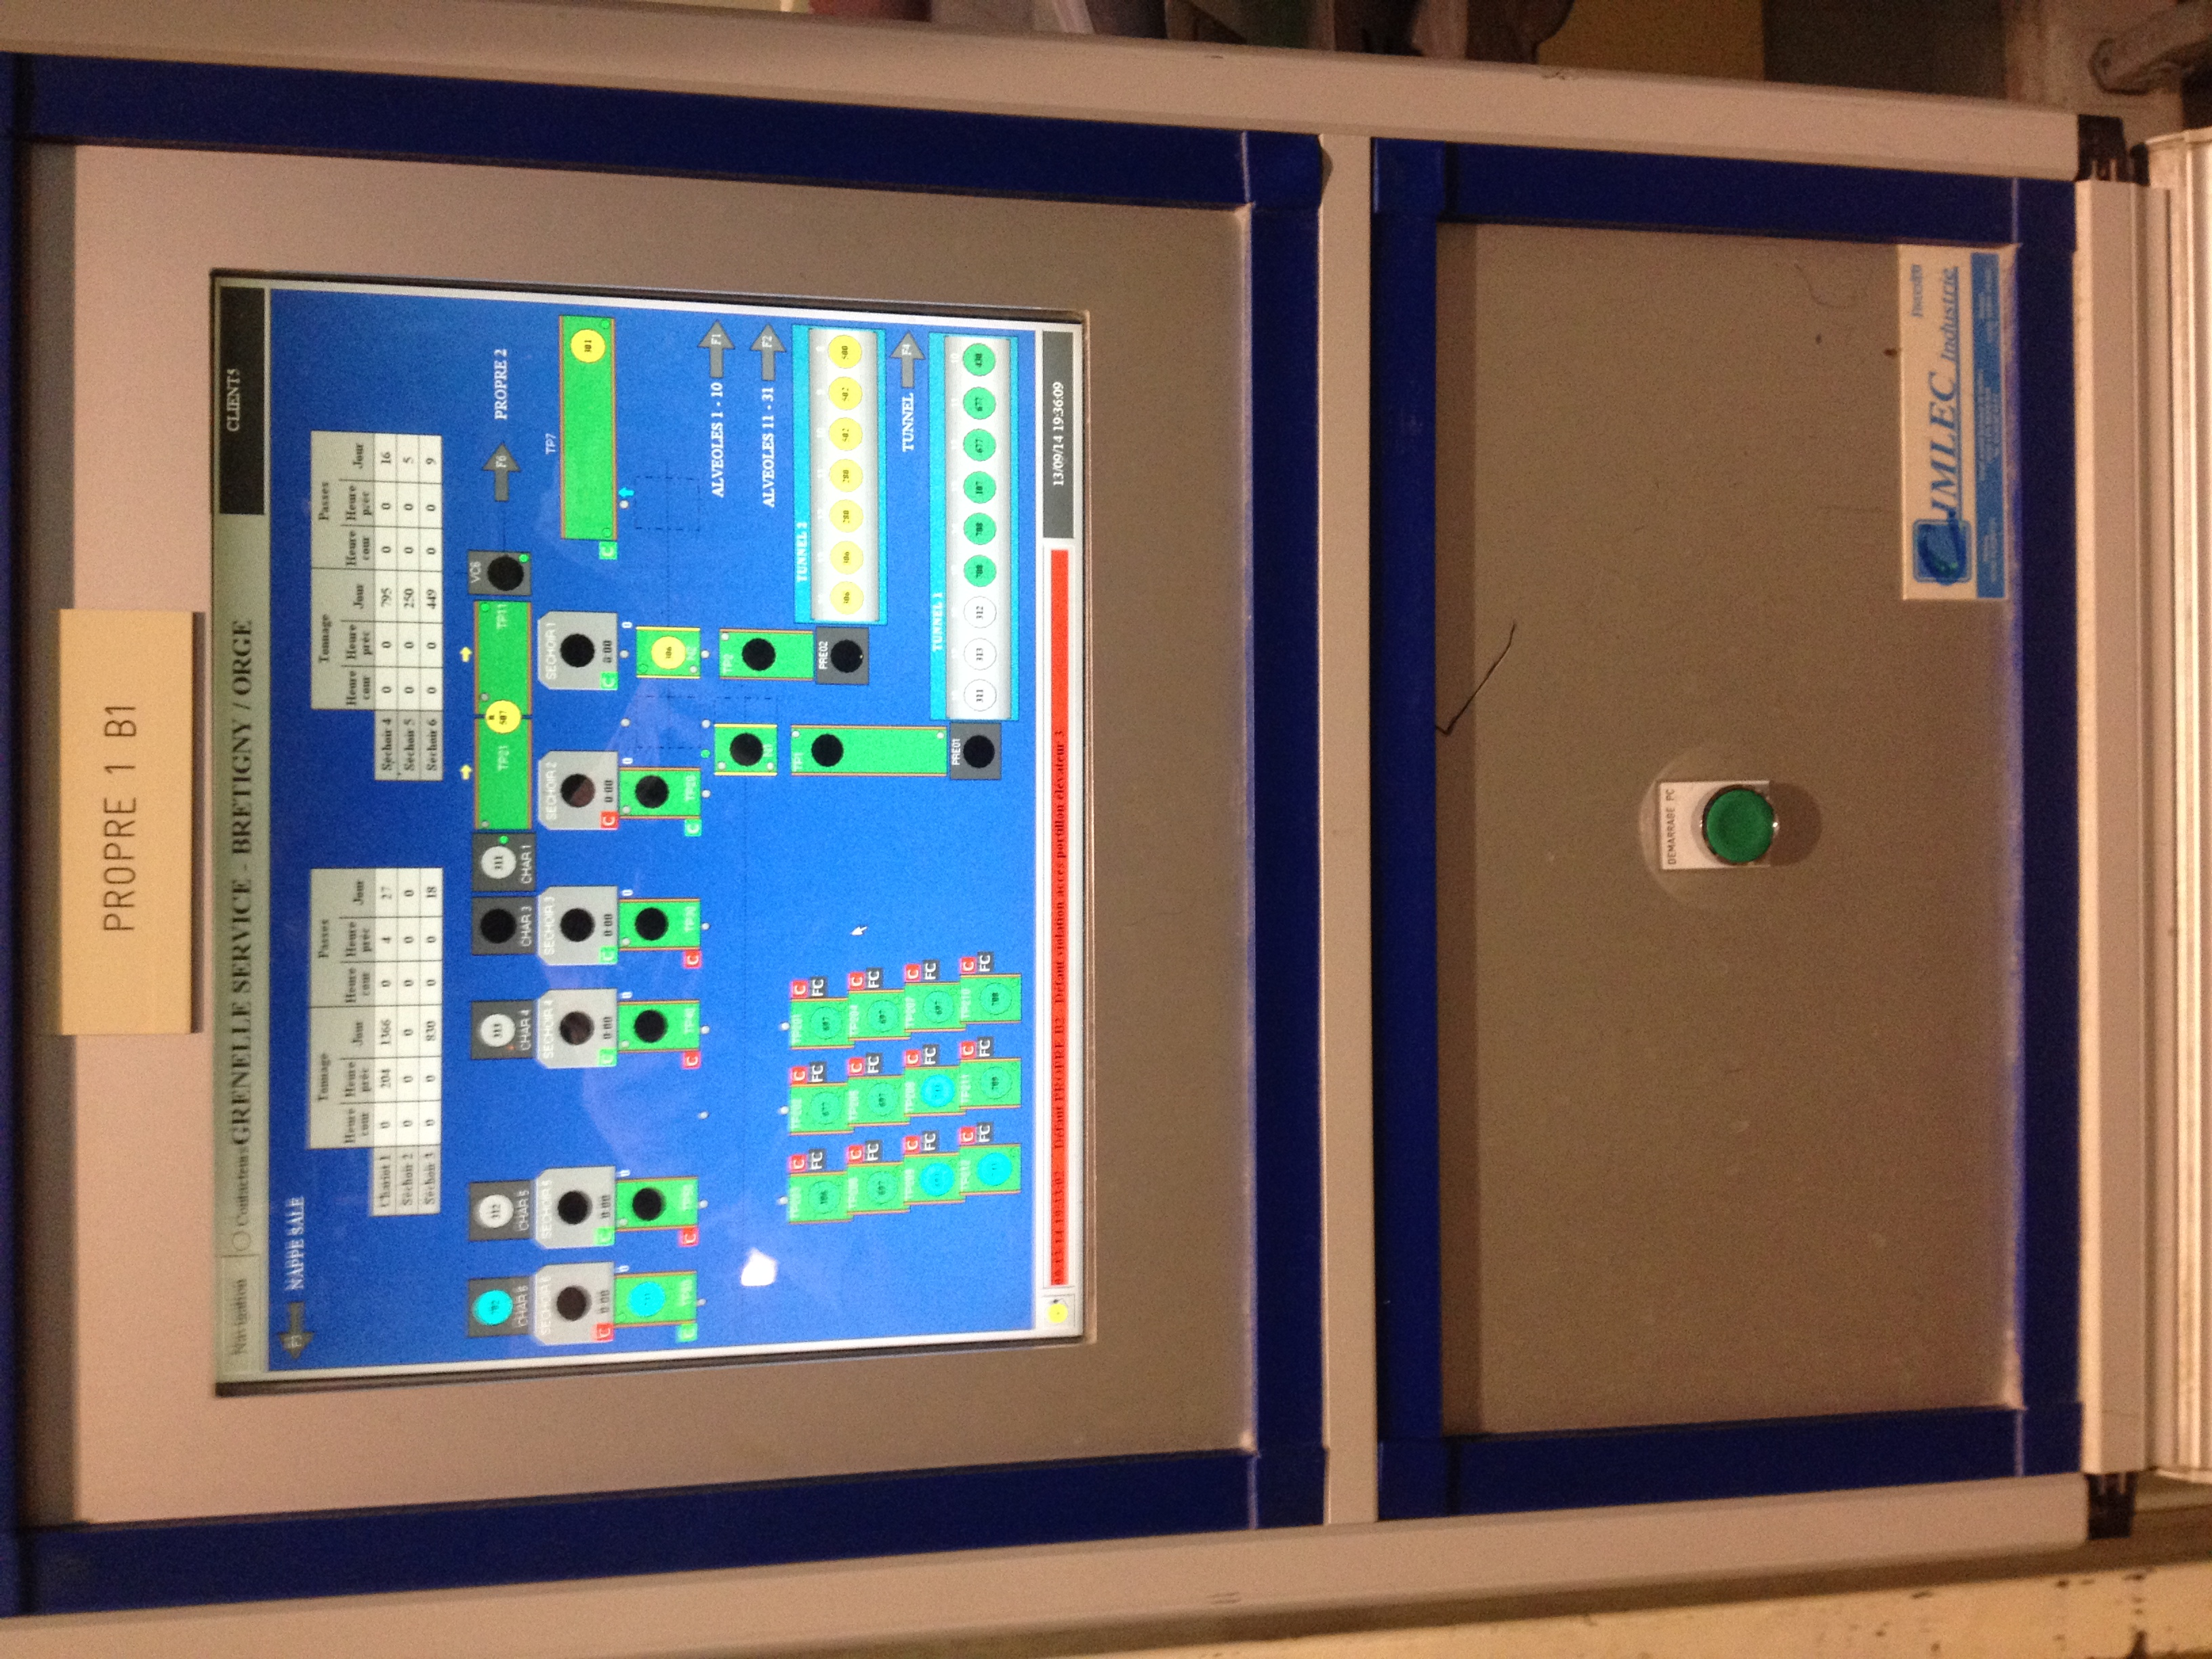
\includegraphics[angle = -90, scale= \rapportFigure]{images/restau_management}
    \caption{Logiciel de management des conteneurs.}
    \label{fig:management}
\end{figure}


\newpage

\section{Réflexions personnelles}

Deux mois se sont enfin passés et nombreuses leçons ont été apprises. Des leçons
de nature professionelle et personnelle  qui vont sûrement m'accompagner pour
toute ma carrière, en France ou au Brésil. Tout d'abord, je profite de 
cette opportunité pour citer un des aspects le plus important à mon avis:
l'organisation. Cette caractéristique est essentielle à toute société qui
souhaite grandir puisqu'elle permet une analyse et une compréhension plus
efficace des données et des résultats. Ainsi, les chefs peuvent prendre des
solutions et décisions plus appropriées sur un problème quelconque. C'est pour
cette raison que j'ai cherché à documenter de façon éclairante toutes
les tâches qui m'ont été confiées, ayant toujours en tête que la réputation du
groupe et le travail de mes collègues dépendaient de mon travail. Il me
faut dire aussi que certaines fois cette qualité manqueait à quelques personnes, ce qui
a rendu mon travail parfois beaucoup plus compliqué par rapport à lui-même
n'ayant pas d'autres interférences.

\vspace{12pt}

Autre aspect très pertinent est la valorisation des personnes qui travaillent
avec moi. Je me suis rendu compte que la qualité du travail réalisé par moi
dépendait de la qualité des activités des autres. Donc, à mon avis, saluer et
se montrer interessé à ce que les autres ont à dire sont aussi importants que
l'efficacité et le savoir faire. Plusieurs fois j'ai regardé certains employés
mettre en question des attitudes des certains chefs précisément par le fait
qu'ils n'ont pas su être polis ou gentils ou ne se sont pas montrés intéressés
au bien-être des opérateurs. Personnellement, une telle personne ne devrait
jamais être choisie pour conduire une équipe, même si elle est capable 
professionnellement: il lui faut d'abord savoir comment respecter les
différentes personnalités. 

\vspace{12pt}

Cette expérience m'a revélé aussi des problèmes. Le premièr, il est celui de la
communication: il me faut encore avancer au français. C'est vrai que je
pouvais me faire compreendre la plupart des temps, mais j'en reconnais que mon
niveau ne suffit pas pour occuper des postes de hautes responsabilités, qui est
l'un des mes projets professionnels. Ma principale difficulté réside à me
socialiser avec les autres. Il me manque ine bonne base de vocabulaires.
C'est pour cette raison que je vais m'engager encore plus à l'apprendissage du
français en deuxième année.

\vspace{12pt}

Le point le plus fort du stage, à mon avis, sont les collègues que j'ai fait
dans tous les secteurs de l'usine. J'ai été vraiment très bien accueilli par tous
qui ont toujours été disponibles pour m'aider à tout moment.
Je confesse qu'au début j'étais un peu inquiet par rapport à l'accueil d'un
étranger et comme serait mon adaptation au travail. Heureusement, tout s'est
très bien passé et maintenant je me trouve plus motivé à poursuivre ma carrière
professionnelle en France et à élargir mon réseau. Par coïncidence, le groupe
venait d'acheter une usine au Brésil lors de mon arrivée, ce qui répresente une
grande opportunité de revenir au groupe dans l'avenir.

\vspace{12pt}

En revanche, je ne peux pas ignorer la partie la plus difficile du stage et
son point negatif: précisément le travail. Tous les jours je pensais aux
perso qui ont passé plusieurs années ou vont passer encore toute
leur vie en faisant les mêmes tâches, très dures dans la plupart de temps,
répétitivement car ils ont des familles à nourrir et ne disposent pas d'études
ou formation académique. C'est un peu triste de penser à cette idée, mais, d'une
certaine façon, cela me motive à continuer et à avancer de plus en plus.
En bref, je pense que le message le plus fort que j'ai pu apprendre, c'est de
valoriser l'éducation et les opportunités qui nous sont données quotidiennement.

%C'est vraiment satisfaisant savoir qu'il y a des personnes prêtes à aider
% n'important laquelle nationalité vous appartenez. Depuis mon arrivée en
% France, j'avais déjà souffert certaines démonstrations d'haine seulement pour
% le fait d'être étranger, ce qui m'a mis en doute si je choisirais la France
% ou pas pour poursuivre ma carrière. Cependant, ce stage m'a rendu motivé
% encore à continuer mon parcours à l'étranger.

\vspace{12pt}

Enfin, je crois que le stage a accompli sa principale mission de me montrer
que, même étant un étranger, je n'ai pas moins de chances qu'un autre
professionnel d'origine française par rapport aux offres d'emploi. C'est
évident que je dois surmonter certains défis culturels, comme la langue
française par exemple, mais c'est avec sûreté que j'affirme qu'une autre porte
s'est ouverte à moi. 

\newpage
\section{Conclusion}

Après avoir fini cette première étape - le stage d'éxécution et généralement
toute ma première année en France - je me sens beaucoup plus préparé à faire
face aux nouveaux défis, vu qu'à ce moment je suis muni d'une base
conceptuelle beaucoup plus concrète par rapport au traitement des
signaux et, de façon générale, l'analyse de systèmes électriques, et d'une
expérience professionnelle assez riche culturellement car j'ai eu la possibité
de connaître de personnes de plusieurs nationalités.

\vspace{12pt}

Bien que le stage n'ait aucun lien avec le domaine que j'ai l'intention de
suivre, c'est très important pour un futur ingénieur qui doit être en contact
avec des secteurs qui pourront éventuellement être administrés par lui.
Par exemple, j'ai pu apercevoir les décisions qu'un chef d'équipe doit prendre
tous les jours, considérant toujours les options qui visent maximiser
l'efficacité. De cette façon, le jeune apprend à valoriser l'effort de ses
opérateurs et comprend que son travail dépend aussi d'eux.

\vspace{12pt}

Le stage est aussi important pour faire attention à la façon d'opération - les
divisions, secteurs, hiérarchie et stratégies -  d'une entreprise, en faisant
référence toujours aux concepts appris en cours. Dans ce contexte, on
considère les principles largement discutés dans les disciplines de première
année comme \og L'organisation de l'entreprise \fg ~et \og Microéconomie \fg ~et
l'electif \og Entreprises innovantes et nouvelle économie \fg. C'est donc une
extension des cours et sûrement cela fait partie du processus d'apprentissage de
l'élève.

\vspace{12pt}

L'objectif principal d'un stage est, à mon avis, aider l'étudiant à décider son
avenir professionnel et à identifier plus facilement les aspects qu'il juge
pouvant être améliorés. C'est alors avec cette idée que je commence la deuxième
année à Supélec avec l'intention de résoudre les questions posées lors de son
déroulement. Dois-je suivre un parcours académique ou plutôt entrepreneurial?
Dans lequel domaine? France ou Brèsil? Je suis sûr que j'aurai leurs résponses à
la fin de cette année, car je sais maintenant le moyen de les chercher.

\vspace{12pt}

Finalement, le stage de fin de première année est une étape fondamentale pour
que l'élève construise son projet professionnel et soit déjà familier au mileau
où il va certainement développer sa carrière.

\end{document}
